%! Auteur = Omar Iskandarani
%! Titel = Wervelklokken en door vorticiteit geïnduceerde zwaartekracht
%! Datum = 23 mei 2025
%! Affiliatie = Onafhankelijk onderzoeker, Groningen, Nederland
%! Licentie = CC-BY 4.0
%! ORCID = 0009-0006-1686-3961

\documentclass[a4paper, aps,preprint,superscriptaddress, 12pt]{revtex4}
\usepackage[paperwidth=210mm, paperheight=297mm, margin=2.5cm]{geometry}
\usepackage{float}
\usepackage{tikz}
\usepackage{makecell}
\usepackage{tabularx}
\usepackage[font=footnotesize]{caption}
\usetikzlibrary{arrows.meta}
\usepackage{pgfplots}
\pgfplotsset{compat=1.18}
\usepackage[none]{hyphenat}
\usepackage{array}
\usepackage{amsmath}
\usepackage{booktabs}
\usepackage[utf8]{inputenc} % Remove if using XeLaTeX or LuaLaTeX
\usepackage{amssymb}
\usepackage{graphicx}
\usepackage{hyperref}
\usepackage{physics}
\usepackage{natbib}
\usepackage{url}
\renewcommand{\arraystretch}{1.5}
\renewcommand{\floatpagefraction}{.8}
\sloppy

\begin{document}
\author{Omar Iskandarani}
\title{
    Wervelingsklokken en door vorticiteit geïnduceerde zwaartekracht:
    Relativiteit herformuleren in een gestructureerde vortex-ether\\
    \textnormal{\normalsize Een topologische vloeistofmechanische benadering van tijdsdilatatie, massa en gravitatie}
}

\date{\today}
\affiliation{Onafhankelijk onderzoeker, Groningen, The Nederland}
\thanks{ORCID: \href{https://orcid.org/0009-0006-1686-3961}{0009-0006-1686-3961}}
\email{info@omariskandarani.com}



\begin{abstract}
Dit artikel presenteert een vloeistofdynamische herformulering van de algemene relativiteit aan de hand van het Vortex Æther Model (VAM), waarin gravitatie en tijdsdilatatie voortkomen uit door vorticiteit geïnduceerde drukgradiënten in een onsamendrukbaar, inviscide superfluïde medium. Binnen een Euclidische ruimte met absolute tijd worden massa en traagheid voorgesteld als topologisch stabiele vortexknopen, waarbij geodetische beweging wordt vervangen door stromingslijnen langs geconserveerde vorticiteitsflux.
Zwaartekracht wordt gemodelleerd als een Bernoulli-potentiaal in vortexvelden, met een bijbehorende veldvergelijking:
\begin{equation*}
    \nabla^2 \Phi_v(\vec{r}) = -\rho_\text{\ae} \|\boldsymbol{\omega}(\vec{r})\|^2
\end{equation*}

en tijdsdilatatie volgt uit lokale vortexenergie:
\begin{equation*}
    \frac{d\tau}{dt} = \sqrt{1 - \frac{C_e^2}{c^2} e^{-r/r_c} - \frac{2G_{\text{swirl}} M_{\text{eff}}(r)}{rc^2} - \beta \Omega^2}
\end{equation*}

VAM introduceert een schaalafhankelijke ætherdichtheid: lokaal (~$10^{18}\,\mathrm{kg/m^3}$) voor kernstabiliteit; macroscopisch (~$10^{-7}\,\mathrm{kg/m^3}$) voor inertievrije interactie. Thermodynamische consistentie wordt bereikt via Clausius-entropie van vortexknopen, wat leidt tot een entropische interpretatie van massa en tijd. Kwantumfenomenen zoals het foto-elektrisch effect en LENR worden opgevat als resonanties binnen vortexnetwerken.

Het model reproduceert Newtonse limieten en frame-dragging als emergente verschijnselen en vormt een toetsbaar, topologisch gegrond alternatief voor klassieke zwaartekrachtmodellen. Deze benadering sluit aan bij eerdere analoge zwaartekrachtprogramma’s~\cite{barcelo2011analogue,volovik2009universe}, maar biedt een fundamenteel hydrodynamisch en knoop-georiënteerd zwaartekrachtraamwerk.
\end{abstract}


\maketitle

\section*{De Æther herzien: van historisch medium naar vorticiteitsveld}

Het begrip \textit{æther} duidde traditioneel op een alles-doordringend medium, noodzakelijk voor golfvoortplanting. Eind negentiende eeuw stelden Kelvin en Tait reeds voor om materie te modelleren als knoopvormige vortexstructuren in een ideale vloeistof~\cite{thomson1867treatise}. Na de nulresultaten van het Michelson--Morley experiment en de opkomst van Einstein's relativiteit verdween het æther-concept uit de mainstream fysica, vervangen door gekromde ruimtetijd. Recentelijk echter is het idee subtiel teruggekeerd in analoge gravitatietheorieën, waarin superfluïde media worden gebruikt om relativistische effecten na te bootsen~\cite{barcelo2011analogue,volovik2009universe}.

Het \textit{Vortex Æther Model} (VAM) herintroduceert de æther expliciet als een topologisch gestructureerd, inviscide superfluïde medium, waarin gravitatie en tijddilatatie niet voortkomen uit geometrische kromming maar uit rotatie-geïnduceerde drukgradiënten en vorticiteitsvelden. De dynamiek van ruimte en materie wordt hierin bepaald door vortex-knopen en behoud van circulatie.

\subsection*{Postulaten van het Vortex Æther Model}

\begin{table}[h!]
    \centering
    \begin{tabular}{rl}
        \midrule
        \hline
        \textbf{1. Continue Ruimte} & Ruimte is Euclidisch, incompressibel en inviscide. \\
        \textbf{2. Geknoopte Deeltjes} & Materie bestaat uit topologisch stabiele vortex-knopen. \\
        \textbf{3. Vorticiteit} & De vortexcirculatie is behouden en gekwantiseerd. \\
        \textbf{4. Absolute Tijd} & Tijd stroomt uniform in de gehele æther. \\
        \textbf{5. Lokale Tijd} & Tijd verloopt lokaal trager door druk- en vorticiteitsgradiënten. \\
        \textbf{6. Zwaartekracht} & Ontstaat uit vorticiteit-geïnduceerde drukgradiënten. \\
        \hline
        \bottomrule
    \end{tabular}
    \caption{Postulaten van het Vortex Æther Model (VAM).}
    \label{tab:postulaten}
\end{table}

De postulaten vervangen ruimtetijdkromming door gestructureerde rotatiestromen en vormen zo het fundament voor emergente massa, tijd, traagheid en zwaartekracht.

\subsection*{Fundamentele VAM-constanten}

\begin{table}[htbp]
    \centering
    \begin{tabular}{llc}
        \hline
        \toprule
        \textbf{Symbool} & \textbf{Naam} & \textbf{Waarde (ca.)} \\
        \hline
        \midrule
        $C_e$ & Tangentiële vortex-kernsnelheid & $1.094 \times 10^6$ m/s \\
        $r_c$ & Vortexkernstraal & $1.409 \times 10^{-15}$ m \\
        $F_{\text{max}}$ & Maximale vortexkracht & $29.05$ N \\
        $\rho_{\ae}$ & Æther-dichtheid & $3.893 \times 10^{18}$ kg/m$^3$ \\
        $\alpha$ & Fijnstructuurconstante ($2 C_e/c$) & $7.297 \times 10^{-3}$\\
        $G_{\text{swirl}}$ & VAM-zwaartekrachtconstante & Afgeleid van $C_e$, $r_c$\\
        $\kappa$ & Circulatie-kwantum ($C_e r_c$) & $1.54 \times 10^{-9}$ m$^2$/s \\
        \hline
        \bottomrule
    \end{tabular}
    \caption{Fundamentele VAM-constanten~\cite{vam2025field}.}
    \label{tab:constants}
\end{table}

\subsection*{Planck-schaal en topologische massa}

Binnen VAM wordt de maximale vortex-interactiekracht expliciet afgeleid uit Planck-schaalfysica:
\[
F_{\text{max}} = \frac{c^4}{4G}\,\alpha\left(\frac{r_c}{L_p}\right)^{-2} = 29.0535~\text{N}
\]

De massa van elementaire deeltjes volgt direct uit topologische vortexknopen, zoals de trefoilknoop ($L_k=3$):
\[
M_e = \frac{8\pi \rho_{\ae} r_c^3}{C_e}\, L_k
\]

Dit verklaart massa en inertie uit topologische knoopstructuren in de æther.

\subsection*{Emergente kwantumconstanten en Schrödingervergelijking}

Plancks constante $\hbar$ ontstaat uit vortex-geometrie en vortexkrachtlimiet:
\[
\hbar = \sqrt{\frac{2M_e F_{\max} r_c^3}{5 \lambda_c C_e}}
\]

Hiermee volgt de Schrödingervergelijking direct uit vortex-dynamica:
\[
i \hbar \frac{\partial \psi}{\partial t} = -\frac{F_{\max} r_c^3}{5 \lambda_c C_e}\nabla^2 \psi + V\psi
\]

\subsection*{LENR en vortex-kwantumeffecten}

In VAM ontstaan lage-energie kernreacties (LENR) uit resonante drukverlaging door vorticiteit-geïnduceerde Bernoulli-effecten. Elektromagnetische interacties en QED-effecten worden herleid tot vortexheliciteit en geïnduceerde vectorpotentialen.

\subsection*{Samenvatting van GR en VAM observabelen}

\begin{table}[h!]
    \centering
    \begin{tabular}{lll}
        \toprule
        \textbf{Observabele} & \textbf{GR-expressie} & \textbf{VAM-expressie} \\
        \midrule
        Tijddilatatie & $\sqrt{1-\frac{2GM}{rc^2}}$ & $\sqrt{1-\frac{\Omega^2 r^2}{c^2}}$\\[0.5em]
        Rodeverschuiving & $z=\left(1-\frac{2GM}{rc^2}\right)^{-1/2}-1$ & $z=\left(1-\frac{v_\phi^2}{c^2}\right)^{-1/2}-1$\\[0.5em]
        Frame-dragging & $\frac{2GJ}{c^2 r^3}$ & $\frac{2G\mu I\Omega}{c^2 r^3}$\\[0.5em]
        Lichtafbuiging & $\frac{4GM}{Rc^2}$ & $\frac{4GM}{Rc^2}$\\
        \bottomrule
    \end{tabular}
    \caption{Vergelijking GR- en VAM-observabelen.}
    \label{tab:vergelijkingen}
\end{table}





\section{Tijdsdilatatie vanuit vortex dynamiek}

We beschouwen een onzichtbare, rotatievrije superfluïde ether met stabiele topologische vortexknopen. Absolute tijd $t_{\text{abs}}$ stroomt met een constante snelheid, terwijl lokale klokken mogelijk een lagere snelheid ervaren als gevolg van drukgradiënten en knoopenergetica. Het Vortex-ethermodel veronderstelt dat de snelheid waarmee tijd in het lokale frame (dichtbij de knoop) stroomt, afhangt van de interne hoekfrequentie $\Omega_k$. In deze sectie leiden we tijddilatatie-analogen af, geïnspireerd door de voorspellingen van de algemene relativiteitstheorie (GR), uitsluitend gebaseerd op druk- en vorticiteitsgradiënten in de vloeistof.

\begin{figure}[htbp]
\centering
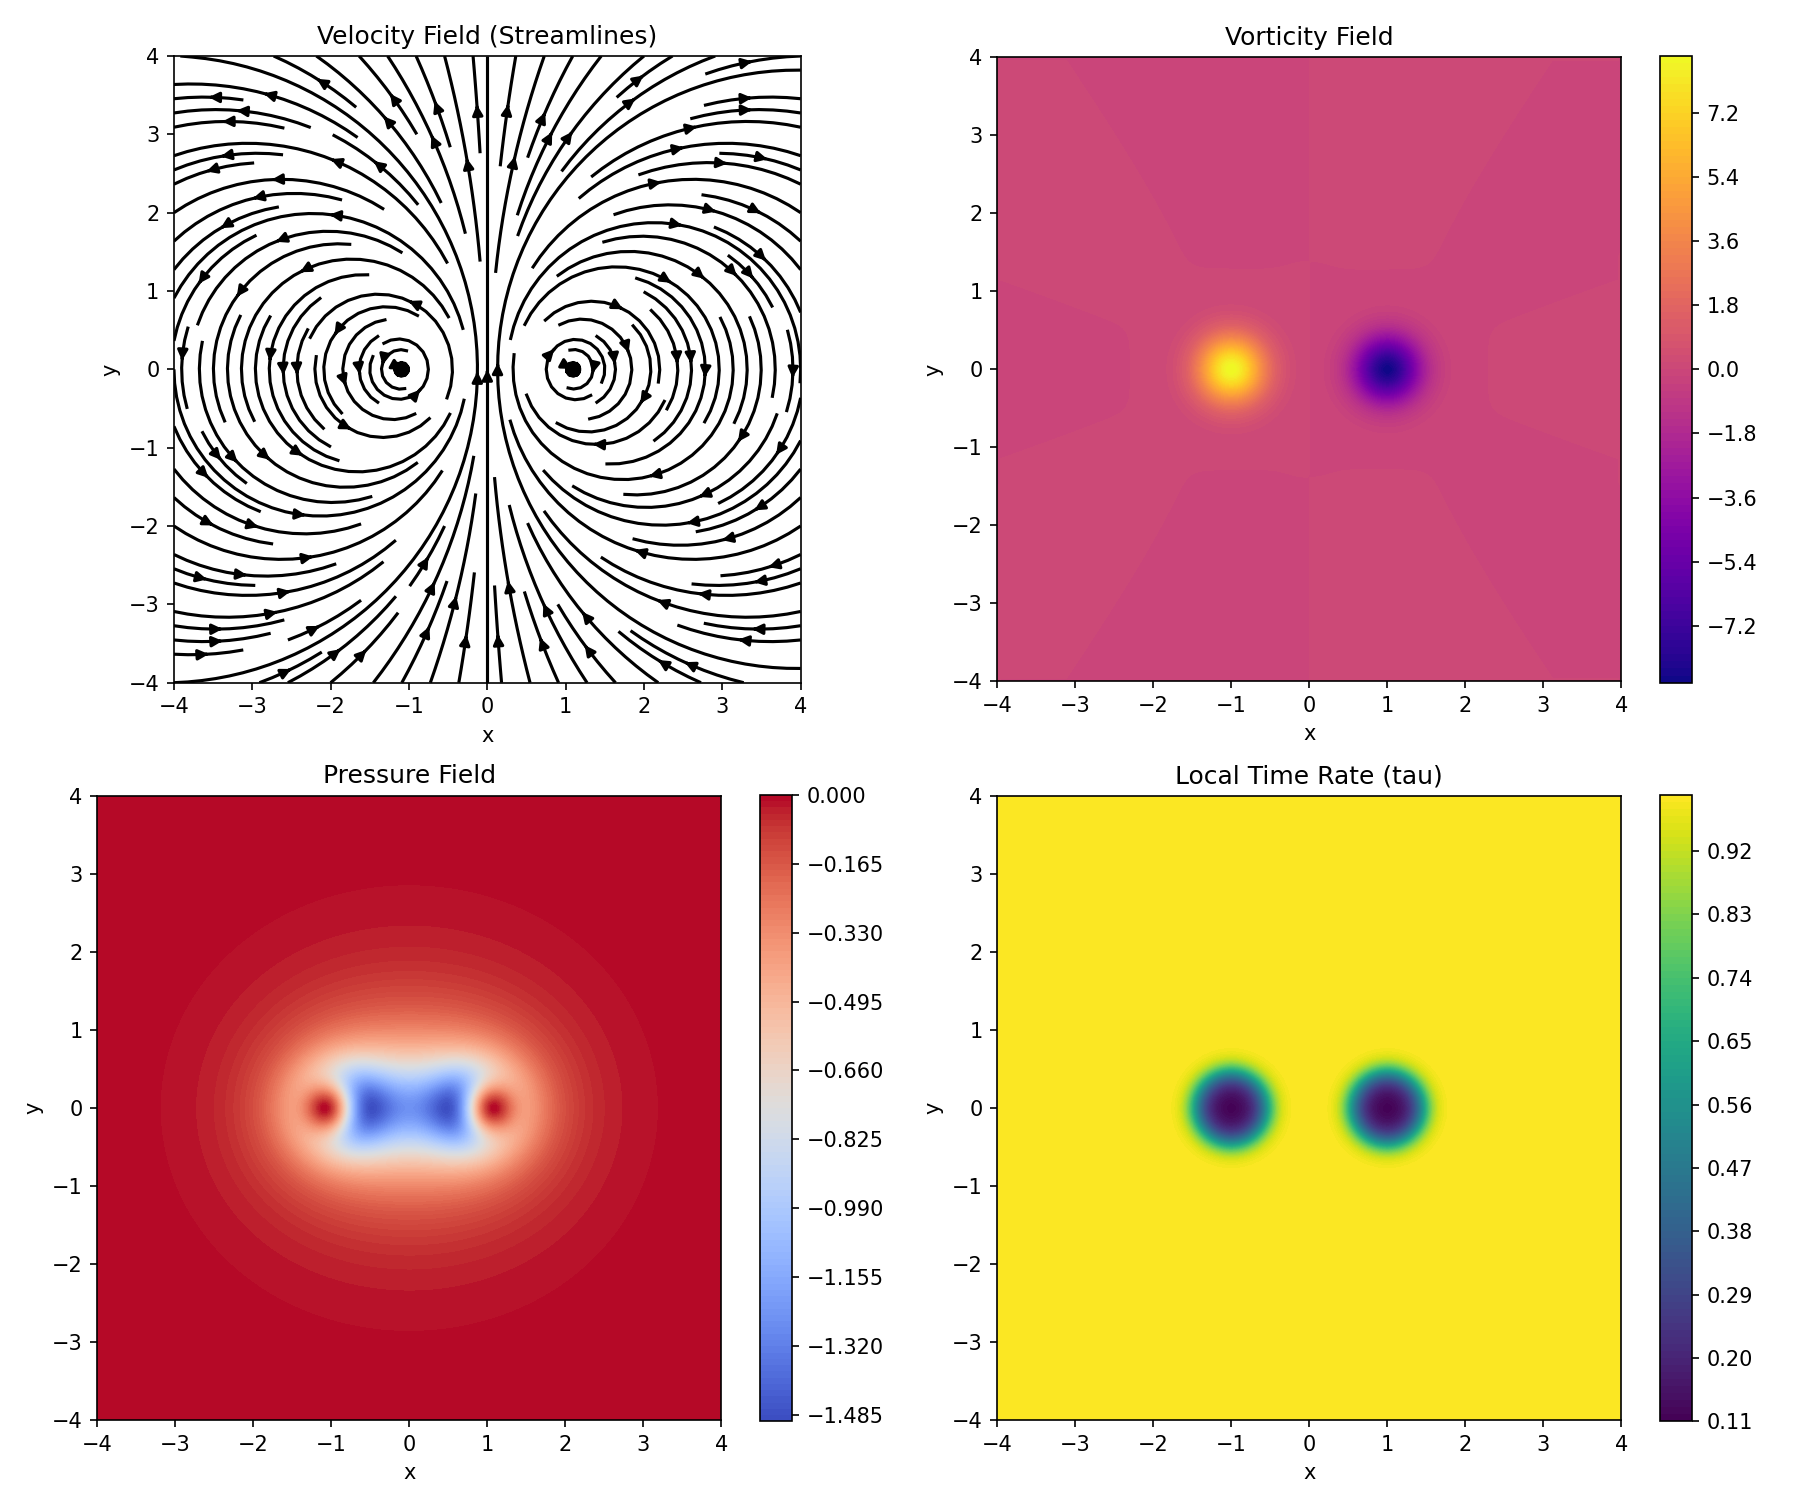
\includegraphics[width=0.85\textwidth]{streamlinesDiPole}
\caption{Snelheid stroomlijnt, vorticiteit, druk en lokale tijdsnelheid $\tau$ voor een gesimuleerd vortexpaar. Het drukminimum en de tijdvertraging komen duidelijk overeen met de gebieden met hoge vorticiteit. Dit illustreert direct de centrale bewering van het ethermodel: tijddilatatie volgt uit vortexenergetica en drukvermindering.}
\label{fig:vortexfields}
\end{figure}

In het Vortex Æther Model (VAM) ontstaat tijdsdilatatie niet vanuit de kromming van ruimtetijd, maar vanuit lokale vortex dynamica. Elk materiedeeltje is in VAM een vortex-knoopstructuur waarvan de interne rotatie (\textit{swirl}) de lokale klokfrequentie beïnvloedt.

De fundamentele koppeling tussen lokale vortex-snelheid en de lokale tijdsmeting volgt uit de Bernoulli-achtige relatie voor drukverlaging in stromingsvelden. De lokale klokfrequentie is gerelateerd aan de vortex-tangentiële snelheid $v_{\phi}(r)$ via de formule:
\begin{equation}\label{eq:vortex_tijdsdilatatie}
    \frac{d\tau}{dt} = \sqrt{1 - \frac{v_{\phi}^2(r)}{c^2}}
\end{equation}

Hierbij is $v_{\phi}(r)$ de tangentiële snelheid van het æthermedium op afstand $r$ tot het centrum van de vortex, en $c$ de lichtsnelheid. Dit is een directe analogie met de speciale relativistische snelheidsafhankelijke tijddilatatie, echter zonder ruimtetijdkromming en louter veroorzaakt door lokale rotatie van het æthermedium.

\subsection{Afleiding vanuit vortex hydrodynamica}

De afleiding volgt uit het Bernoulli-principe voor een ideale vloeistofstroming, gegeven door:
\begin{equation}\label{eq:Bernoulli}
    P + \frac{1}{2}\rho_{\ae} v^2 = \text{constant}
\end{equation}

Met vortex-stroming geïntroduceerd via vorticiteit $\vec{\omega} = \nabla \times \vec{v}$, definieert de lokale drukverlaging ten opzichte van de verre omgeving een lokale tijdvertraging. De lokale vortexsnelheid is gegeven door:
\begin{equation}\label{eq:tangentiele_snelheid}
    v_{\phi}(r) = \frac{\Gamma}{2\pi r} = \frac{\kappa}{r}
\end{equation}

waarbij $\Gamma$ de circulatieconstante is, en $\kappa$ het circulatiekwantum. Substitutie van \eqref{eq:tangentiele_snelheid} in \eqref{eq:vortex_tijdsdilatatie} geeft expliciet:
\begin{equation}\label{eq:vortex_tijd_expliciet}
    \frac{d\tau}{dt} = \sqrt{1 - \frac{\kappa^2}{c^2 r^2}}
\end{equation}

Hiermee is de tijdsdilatatie expliciet uitgedrukt in fundamentele vortex-parameters.

\subsection{Vergelijking met algemene relativiteit}

Ter vergelijking, in algemene relativiteit (GR) ontstaat gravitationele tijddilatatie uit ruimtetijdkromming, uitgedrukt door de Schwarzschildmetriek~\cite{schutz2009first}:
\begin{equation}\label{eq:GRtijd}
    \frac{d\tau}{dt} = \sqrt{1 - \frac{2GM}{rc^2}}
\end{equation}

De overeenkomsten en verschillen zijn direct zichtbaar: GR's gravitationele tijddilatatie is gerelateerd aan massa $M$ en gravitatieconstante $G$, terwijl VAM tijdsdilatatie puur hydrodynamisch is en direct verbonden met de lokale rotatiesnelheid van het æthermedium via vortex-circulatie $\kappa$.

\begin{figure}[ht!]
    \centering
    % Plaats hier een eigen grafiek of illustratie.
    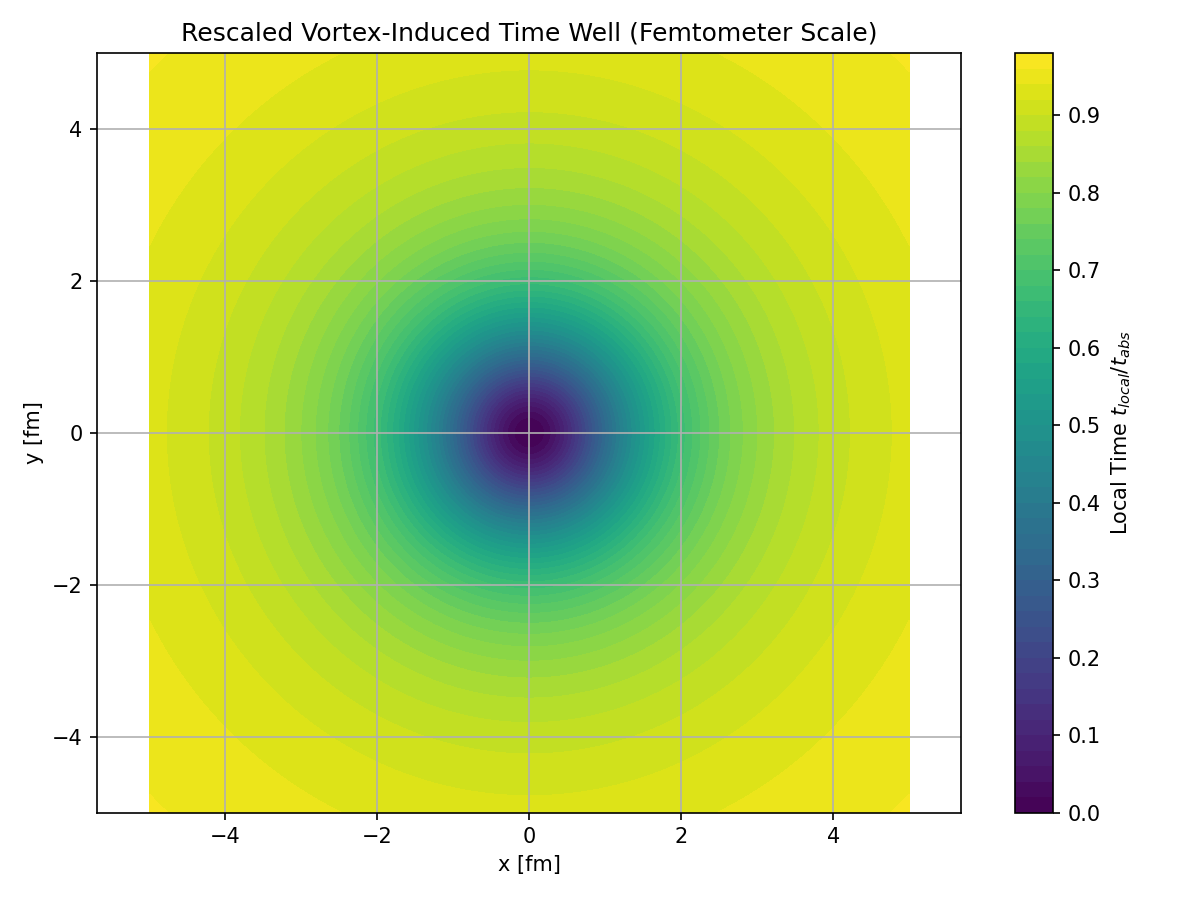
\includegraphics[width=0.7\linewidth]{RadialProfileOfLocalTimeDilation_Vortex-Induced_Time_Well}
    \caption{Vergelijking tussen VAM- (vortex dynamiek) en GR-tijdsdilatatie, als functie van afstand tot vortexkern en Schwarzschildradius.}
    \label{fig:vergelijking_VAMGR}
\end{figure}

In Figuur~\ref{fig:vergelijkingVAMGR} zien we dat de VAM-tijdsdilatatie functioneel vergelijkbaar is met GR-prediction bij voldoende afstand. Bij afnemende afstand (nabij vortexkern of Schwarzschildradius) ontstaan verschillen door vortex-specifieke effecten en topologische knoopstructuren.

Samenvattend vervangt het VAM ruimtetijdkromming door werveldynamica, met behoud van meetbare tijddilatatie-effecten die overeenstemmen met gevestigde experimentele resultaten zoals Hafele–Keating~\cite{hafele1972around}, maar vanuit een fundamenteel andere fysische verklaring.


Ter illustratie vergelijken we in Figuur~\ref{fig:vergelijkingVAMGR} VAM en GR expliciet voor een neutronenster met $M = 2\,M_\odot$ en radius $R = 10\,\text{km}$. De verschillen worden duidelijk nabij de oppervlakte van het object, waar vortex-specifieke effecten optreden.

\begin{figure}[ht!]
    \centering
    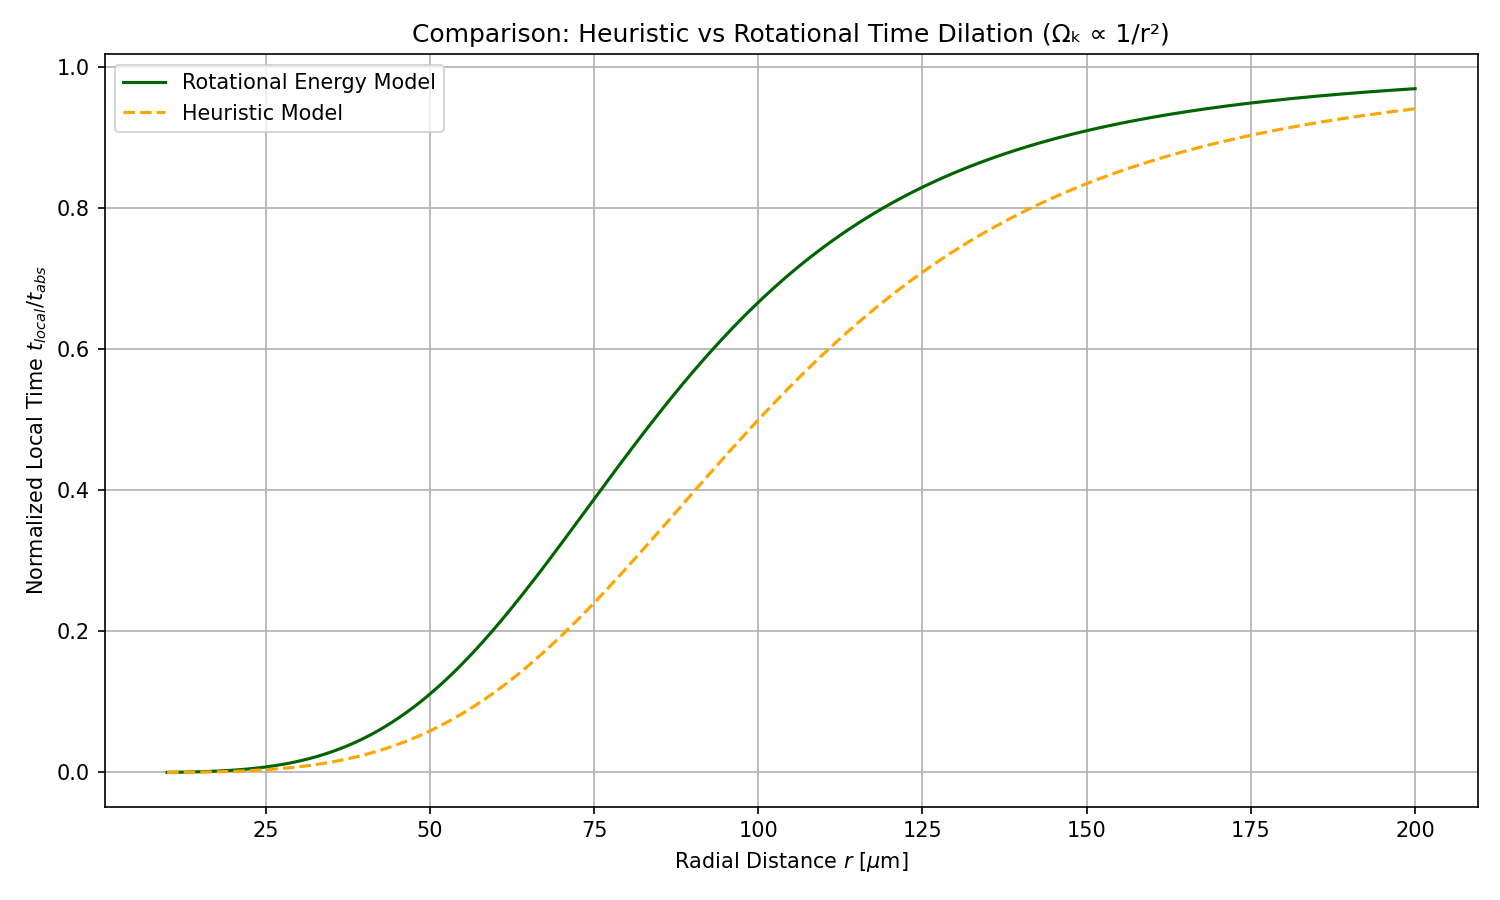
\includegraphics[width=0.7\linewidth]{RotationalVsHeuristicTimeDilation}
    \caption{Verschil tussen VAM en GR-tijddilatatie voor een neutronenster ($2\,M_\odot$, $R=10$ km).}
    \label{fig:vergelijkingVAMGR}
\end{figure}

\subsection{Interpretatie van schaalafhankelijke ætherdichtheid}

VAM gebruikt een schaalafhankelijke ætherdichtheid: lokaal zeer hoog ($\sim10^{18}$ kg/m³) voor kernstabiliteit en macroscopisch laag ($\sim10^{-7}$ kg/m³) om inertievrije propagatie van interacties mogelijk te maken. De hoge dichtheid in vortexkernen versterkt lokaal de vortexsnelheid en daarmee de tijddilatatie significant, terwijl macroscopisch juist minimale weerstand voor propagatie van effecten geboden wordt.

\subsection{Praktische implicaties en experimentele toetsbaarheid}

Een praktische implicatie van vortex-geïnduceerde tijddilatatie is dat klokken dicht bij intense vortexvelden meetbaar trager zouden lopen. Dit kan theoretisch getoetst worden met ultra-precieze atoomklokken in laboratorium vortexexperimenten, of indirect via astrofysische observaties van pulsars en neutronensterren. Het Hafele–Keating experiment biedt een directe analogie voor tijddilatatie door beweging en hoogteverschillen, die in VAM overeenkomt met lokale vortexvariaties~\cite{hafele1972around}.


\section{Entropie en quantum-effecten in het Vortex Æther Model}

Het Vortex Æther Model (VAM) biedt een mechanistische basis voor zowel thermodynamische als kwantummechanische fenomenen, niet door postulaten over abstracte toestandsruimten, maar via de dynamica van knopen en wervels in een superfluïde æther. Twee centrale begrippen—entropie en kwantisatie—worden in VAM afgeleid uit respectievelijk vorticiteitverdeling en knottopologie.

\subsection{Entropie als vorticiteit-verdeling}

In thermodynamica is entropie $S$ een maat voor de interne energieverdeling of wanorde. In VAM ontstaat entropie niet als statistisch fenomeen, maar uit ruimtelijke variaties in werveling (vorticiteit). Voor een wervelconfiguratie $V$ wordt de entropie gegeven door:

\begin{equation}
S \propto \int_V \|\vec{\omega}\|^2 \, dV,
\end{equation}

waar $\vec{\omega} = \nabla \times \vec{v}$ de lokale vorticiteit is. Dit betekent:

\begin{itemize}
    \item \textbf{Meer rotatie = meer entropie}: Regio's met sterke swirl dragen bij aan verhoogde entropie.
    \item \textbf{Thermodynamisch gedrag ontstaat uit werveluitzetting}: Bij toevoer van energie (warmte), zet de wervelgrens uit, de swirl neemt af en $S$ stijgt—analogie met gasexpansie.
\end{itemize}

Deze interpretatie verbindt Clausius’ warmtetheorie met æthermechanica: warmte is equivalent aan verhoogde swirlverspreiding.

\subsection{Quantumgedrag uit geknoopte wervelstructuren}

Kwantumverschijnselen zoals discrete energieniveaus, spin, en golf-deeltje-dualiteit vinden in VAM hun oorsprong in topologisch geconserveerde wervelknopen:

\begin{itemize}
    \item \textbf{Circulatiequantisatie:}
    \begin{equation}
    \Gamma = \oint \vec{v} \cdot d\vec{l} = n \cdot \kappa,
    \end{equation}
    waarbij $\kappa = h/m$ en $n \in \mathbb{Z}$ het windinggetal is.
    \item \textbf{Hele getallen ontstaan uit knottopologie:} De helixstructuur van een wervelknoop (zoals een trefoil) zorgt voor discrete toestanden met bepaalde linking numbers $L_k$.
    \item \textbf{Heliciteit als spin-analoog:}
    \begin{equation}
    H = \int \vec{v} \cdot \vec{\omega} \, dV,
    \end{equation}
    waarbij $H$ invariant is onder ideale stroming, net zoals spin geconserveerd is in quantummechanica.
\end{itemize}

\subsection{VAM-interpretatie van kwantisatie en dualiteit}

In plaats van abstracte Hilbertruimten beschouwt VAM een deeltje als een stabiele knoop in het ætherveld. Deze wervelconfiguratie bezit:

\begin{itemize}
    \item Een \textbf{kern} (knooplichaam) met quantumsprongen (resonanties).
    \item Een \textbf{uiterlijk veld} dat als golf fungeert (zoals de Schrödinger-golf).
    \item Een \textbf{heliciteit} die gedraagt als interne vrijheidsgraden (bijv. spin).
\end{itemize}

Het golf-deeltje-dualisme komt zo voort uit het feit dat knopen zowel gelokaliseerd (kern) als uitgesmeerd (veld) zijn.

\subsection{Samenvattend}

VAM biedt dus een coherente, vloeistofmechanische oorsprong voor zowel:

\begin{enumerate}
    \item \textbf{Thermodynamica:} Entropie ontstaat uit swirlverdeling.
    \item \textbf{Quantummechanica:} Kwantisatie en dualiteit zijn emergente eigenschappen van geknoopte wervel topologieën.
\end{enumerate}

Deze benadering laat zien dat kwantum- en thermodynamische fenomenen niet fundamenteel verschillend zijn, maar voortkomen uit hetzelfde wervelmechanisme op verschillende schalen.


\section{Tijdsmodulatie door rotatie van wervelknopen}

Voortbouwend op de behandeling van tijdsdilatatie via druk en Bernoulli-dynamica in de vorige sectie, richten we ons nu op de intrinsieke rotatie van topologische wervelknopen. In het Vortex Æther Model (VAM) worden deeltjes gemodelleerd als stabiele, topologisch behouden wervelknopen ingebed in een onsamendrukbaar, niet-viskeus superfluïde medium. Elke knoop bezit een karakteristieke interne hoekfrequentie $\Omega_k$, en deze interne beweging induceert lokale tijdmodulatie ten opzichte van de absolute tijd van de æther.

In plaats van het krommen van de ruimtetijd, stellen we voor dat interne rotatie-energie en heliciditeitsbehoud temporele vertragingen veroorzaken die analoog zijn aan gravitationele roodverschuiving. In deze sectie worden deze ideeën uitgewerkt met behulp van heuristische en energetische argumenten die consistent zijn met de hiërarchie die in Sectie I is geïntroduceerd.

\subsection{Heuristische en energetische afleiding}

We beginnen met het voorstellen van een rotatiegeïnduceerde tijdsdilatatieformule op basis van de interne hoekfrequentie van de knoop:

\begin{equation}
\frac{t_{\text{local}}}{t_{\text{abs}}} = \left(1 + \beta \Omega_k^2 \right)^{-1}\label{eq:rotational_induced_time_dilation}
\end{equation}

waarbij:

\begin{itemize}
\item $t_{\text{local}}$ de eigentijd nabij de knoop is,
\item $t_{\text{abs}}$ de absolute tijd van de achtergrond-æther is,
\item $\Omega_k$ de gemiddelde kernhoekfrequentie is frequentie,
\item $\beta$ is een koppelingscoëfficiënt met dimensies $[\beta] = \text{s}^2$.
\end{itemize}

Voor kleine hoeksnelheden verkrijgen we een eerste-orde-expansie:

\begin{equation}
\frac{t_{\text{local}}}{t_{\text{abs}}} \approx 1 - \beta \Omega_k^2 + \mathcal{O}(\Omega_k^4)\label{eq:rotational_induced_time_dilation_expansion}
\end{equation}

Deze vorm loopt parallel met de Lorentzfactor bij lage snelheden in de speciale relativiteitstheorie:

\begin{equation}
\frac{t_{\text{moving}}}{t_{\text{rest}}} \approx 1 - \frac{v^2}{2c^2}\label{eq:parallels_lorentz_time_dilation}
\end{equation}

Dit levert een belangrijke analogie op: Interne rotatiebeweging in VAM induceert tijdvertraging, vergelijkbaar met hoe translationele snelheid tijddilatatie induceert in SR.

Om de fysische basis van deze uitdrukking te versterken, relateren we tijddilatatie nu aan de energie die is opgeslagen in wervelrotatie. Stel dat de wervelknoop een effectief traagheidsmoment $I$ heeft. De rotatie-energie wordt gegeven door:

\begin{equation}
E_{\text{rot}} = \frac{1}{2} I \Omega_k^2\label{eq:rotational_energy_inertia}
\end{equation}

Aannemende dat de tijd vertraagt door deze energiedichtheid, schrijven we:

\begin{equation}
\frac{t_{\text{local}}}{t_{\text{abs}}} = \left(1 + \beta E_{\text{rot}} \right)^{-1} = \left(1 + \frac{1}{2} \beta I \Omega_k^2 \right)^{-1}\label{eq:time_dilation_rotational_energy_inertia}
\end{equation}

Deze uitdrukking dient als de energetische analoog van het op druk gebaseerde Bernoulli-model uit Sectie I (zie vgl. ~\eqref{eq:vortex_tijdsdilatatie}). Het ondersteunt de interpretatie van wervel-geïnduceerde tijdsputten via energieopslag in plaats van geometrische deformatie.

\subsection{Topologische en fysische rechtvaardiging}

Topologische wervelknopen worden niet alleen gekenmerkt door rotatie, maar ook door heliciteit:

\begin{equation}
H = \int \vec{v} \cdot \vec{\omega} \, d^3x \label{eq:helicity_rotation}
\end{equation}

Heliciteit is een behouden grootheid in ideale (onzichtbare, onsamendrukbare) vloeistoffen, die de verbinding en draaiing van wervellijnen codeert. De rotatiefrequentie $\Omega_k$ wordt een topologisch betekenisvolle indicator van de identiteit en dynamische toestand van de knoop.

Hogere $\Omega_k$-waarden duiden op meer rotatie-energie en diepere drukputten, wat leidt tot tijdelijke vertragingen die lijken op gravitationele roodverschuiving, maar zonder dat er sprake is van ruimtetijdkromming.

Elk deeltje is een topologische wervelknoop:
\begin{itemize}
\item Lading $\leftrightarrow$ draaiing of chiraliteit van de knoop
\item Massa $\leftrightarrow$ geïntegreerde vorticiteitsenergie
\item Spin $\leftrightarrow$ knoophelix:
\end{itemize}
Stabiliteit $\leftrightarrow$ knooptype (Hopf-verbindingen, Trefoil, enz.) en energieminimalisatie in de wervelkern

Dit model:

\begin{itemize}
\item Schrijft tijdmodulatie toe aan behouden, intrinsieke rotatie-energie,
\item Vereist geen externe referentiekaders (absolute æthertijd is universeel),
\item Behoudt temporele isotropie buiten de wervelkern,
\item Biedt een natuurlijke vervanging voor de ruimtetijdkromming van GR. \end{itemize}

Daarom biedt dit wervel-energetische tijdsdilatatieprincipe een krachtig alternatief voor relativistische tijdmodulatie door alle temporele effecten te verankeren in rotatie-energetica en topologische invarianten.

In de volgende sectie zullen we laten zien hoe deze ideeën metriekachtig gedrag reproduceren voor roterende waarnemers, inclusief een directe vloeistofmechanische analoog aan de Kerr-metriek van de algemene relativiteitstheorie.
\section{Eigen tijd voor een roterende waarnemer in ætherstroming}

Nu we tijddilatatie hebben vastgesteld in het Vortex Æther Model (VAM) door middel van druk, hoeksnelheid en rotatie-energie, breiden we ons formalisme nu uit naar roterende waarnemers. Deze sectie toont aan dat vloeistofdynamische tijdmodulatie in VAM uitdrukkingen kan reproduceren die structureel vergelijkbaar zijn met die afgeleid uit de algemene relativiteitstheorie (GR), met name in axiaal symmetrische roterende ruimtetijden zoals de Kerr-geometrie. VAM bereikt dit echter zonder ruimtetijdkromming aan te roepen. In plaats daarvan wordt tijdmodulatie volledig bepaald door kinetische variabelen in het ætherveld.

\subsection{GR-propertijd in roterende frames}

In de algemene relativiteitstheorie wordt de eigentijd \(d\tau\) voor een waarnemer met hoeksnelheid \(\Omega_\text{eff}\) in een stationaire, axiaal symmetrische ruimtetijd gegeven door:

\begin{equation}
\left( \frac{d\tau}{dt} \right)^2_\text{GR} = -\left[ g_{tt} + 2g_{t\varphi} \Omega_\text{eff} + g_{\varphi\varphi} \Omega_\text{eff}^2 \right]
\label{eq:GR_proper_time}
\end{equation}

waarbij \(g_{\mu\nu}\) componenten zijn van de ruimtetijdmetriek (bijv. in Boyer-Lindquist coördinaten voor Kerr-ruimtetijd). Deze formulering houdt rekening met zowel gravitationele roodverschuiving als rotatie-effecten (frame-dragging).

\subsection{Æther-gebaseerde analogie: Snelheidsafgeleide tijdmodulatie}

In VAM is de ruimtetijd niet gekromd. Waarnemers bevinden zich in plaats daarvan in een dynamisch gestructureerde æther waarvan de lokale stroomsnelheden de tijddilatatie bepalen. Laat de radiale en tangentiële componenten van de æthersnelheid zijn:

\begin{itemize}
\item \(v_r\): radiale snelheid,
\item \(v_\varphi = r\Omega_k\): tangentiële snelheid als gevolg van lokale wervelrotatie,
\item \(\Omega_k = \frac{\kappa}{2\pi r^2}\): lokale hoeksnelheid (met \(\kappa\) als circulatie).
\end{itemize}

We postuleren een correspondentie tussen GR-metrische componenten en andere snelheidstermen:

\begin{equation}
\begin{aligned}
g_{tt} &\rightarrow -\left(1 - \frac{v_r^2}{c^2}\right), \\
g_{t\varphi} &\rightarrow -\frac{v_r v_\varphi}{c^2}, \\
g_{\varphi\varphi} &\rightarrow -\frac{v_\varphi^2}{c^2 r^2}
\end{aligned}
\label{eq:VAM_metric_terms}
\end{equation}

Door deze in de GR-expressie voor de juiste tijd te substitueren, verkrijgen we de VAM-gebaseerde analoog:

\begin{equation}
\left( \frac{d\tau}{dt} \right)^2_\text{\ae} = 1 - \frac{v_r^2}{c^2} - \frac{2v_r v_\varphi}{c^2} - \frac{v_\varphi^2}{c^2}
\label{eq:VAM_proper_time}
\end{equation}

De termen combineren:

\begin{equation}
\left( \frac{d\tau}{dt} \right)^2_\text{\ae} = 1 - \frac{1}{c^2}(v_r + v_\varphi)^2
\label{eq:VAM_proper_time_combined}
\end{equation}

Deze formulering reproduceert gravitationele en frame-dragging tijdseffecten puur uit de ætherdynamica: $\langle \omega^2 \rangle$ speelt de rol van gravitationele roodverschuiving en circulatie $\kappa$ codeert rotatieweerstand. Deze benadering sluit aan bij recente vloeistofdynamische interpretaties van zwaartekracht en tijd \cite{barcelo2011analogue}, \cite{fedi2017gravity}.
Dit model gaat momenteel uit van rotatievrije stroming buiten knopen en verwaarloost viscositeit, turbulentie en kwantumcompressibiliteit. Toekomstige uitbreidingen kunnen gekwantiseerde circulatiespectra of grenseffecten in beperkte æthersystemen omvatten.

\begin{equation}
\boxed{\left( \frac{d\tau}{dt} \right)^2_\text{\ae} = 1 - \frac{1}{c^2}(v_r + r\Omega_k)^2}
\label{eq:VAM_proper_time_final}
\end{equation}

\subsection{Fysische interpretatie en modelconsistentie}

Dit resultaat in het kader weerspiegelt de GR-uitdrukking voor roterende waarnemers, maar komt strikt voort uit de klassieke vloeistofdynamica. Het laat zien dat naarmate de lokale æthersnelheid de lichtsnelheid nadert – door radiale instroom of rotatiebeweging – de eigentijd vertraagt. Dit impliceert het bestaan van "tijdputten" waar de kinetische energiedichtheid domineert.

Belangrijkste observaties:

\begin{itemize}
\item Bij afwezigheid van radiale stroming (\(v_r = 0\)) ontstaat tijdvertraging volledig door wervelrotatie.
\item Wanneer zowel \(v_r\) als \(\Omega_k\) aanwezig zijn, verlaagt de cumulatieve snelheid de lokale tijdssnelheid.
\item Deze uitdrukking komt overeen met het energetische model van Sectie II als we \(v_r + r\Omega_k\) interpreteren als een bijdrage aan de lokale energiedichtheid.
\end{itemize}

In het VAM-kader komt de structuur van de eigentijd van de waarnemer dus voort uit ætherische stromingsvelden. Dit bevestigt dat GR-achtig temporeel gedrag kan ontstaan in een vlakke, Euclidische 3D-ruimte met absolute tijd, volledig bepaald door gestructureerde vorticiteit en circulatie.

In het volgende gedeelte onderzoeken we hoe VAM deze overeenkomst uitbreidt naar gravitatiepotentialen en frame-dragging-effecten via circulatie en vorticiteitsintensiteit, en zo een analogie vormt voor de Kerr-tijd-roodverschuivingsformule.
\section{Kerr-achtige tijdsaanpassing op basis van vorticiteit en circulatie}

Om de analogie tussen de algemene relativiteitstheorie (GR) en het wervel-æthermodel (VAM) te voltooien, leiden we nu een tijdmodulatieformule af die de roodverschuiving en frame-dragging-structuur in de Kerr-oplossing weerspiegelt. In GR beschrijft de Kerr-metriek de ruimtetijdgeometrie rond een roterende massa en voorspelt zowel gravitationele tijddilatatie als frame-dragging als gevolg van impulsmoment. VAM legt vergelijkbare verschijnselen vast via de dynamiek van gestructureerde vorticiteit en circulatie in de æther, zonder dat ruimtetijdkromming nodig is.

\subsection{Algemene relativistische Kerr-roodverschuivingsstructuur}

In de GR-Kerr-metriek wordt de eigentijd $d\tau$ voor een waarnemer nabij een roterende massa beïnvloed door zowel massa-energie als impulsmoment. Een vereenvoudigde benadering voor de tijddilatatiefactor nabij een roterend lichaam is:
\begin{equation}
t_\text{adjusted} = \Delta t \cdot \sqrt{1 - \frac{2GM}{rc^2} - \frac{J^2}{r^3c^2}}
\label{eq:Kerr_time_dilation}
\end{equation}
waarbij:
\begin{itemize}
\item $M$: massa van het roterende lichaam,
\item $J$: impulsmoment,
\item $r$: radiale afstand tot de bron,
\item $G$: gravitatieconstante van Newton,
\item $c$: lichtsnelheid.
\end{itemize}

De eerste term correspondeert met gravitationele roodverschuiving ten opzichte van de massa, terwijl de tweede rekening houdt met rotatie-effecten (frame-dragging).

\subsection{Æther analoog via vorticiteit en circulatie}

In VAM drukken we gravitatieachtige invloeden uit via vorticiteitsintensiteit $\langle \omega^2 \rangle$ en totale circulatie $\kappa$. Deze worden geïnterpreteerd als:
\begin{itemize}
\item $\langle \omega^2 \rangle$: gemiddelde kwadratische vorticiteit over een gebied,
\item $\kappa$: behouden circulatie, coderend voor impulsmoment.
\end{itemize}

We definiëren de æthergebaseerde analoog door de volgende vervangingen uit te voeren:
\begin{equation}
\begin{aligned}
\frac{2GM}{rc^2} &\rightarrow \frac{\gamma \langle \omega^2 \rangle}{rc^2}, \\
\frac{J^2}{r^3c^2} &\rightarrow \frac{\kappa^2}{r^3c^2}
\end{aligned}
\label{eq:Kerr_replacements}
\end{equation}

Hier is $\gamma$ een koppelingsconstante die de vorticiteit relateert aan de effectieve zwaartekracht (analoog aan $G$). De op æther gebaseerde eigentijd wordt dan:

\begin{equation}
\boxed{t_\text{adjusted} = \Delta t \cdot \sqrt{1 - \frac{\gamma \langle \omega^2 \rangle}{rc^2} - \frac{\kappa^2}{r^3c^2}}}
\label{eq:Kerr_time_dilation_ae}
\end{equation}

Dit weerspiegelt de Kerr-roodverschuiving en frame-dragging-structuur met behulp van vloeistofdynamische variabelen. In deze afbeelding:
\begin{itemize}
\item $\langle \omega^2 \rangle$ speelt de rol van energiedichtheid die gravitationele roodverschuiving produceert,
\item $\kappa$ vertegenwoordigt impulsmoment dat tijdelijke frame-dragging genereert,
\item De vergelijking reduceert tot een vlakke æthertijd ($t_\text{aangepast} \to \Delta t$) wanneer beide termen verdwijnen.
\end{itemize}


\subsection*{Hybride VAM Frame-Dragging Hoeksnelheid}


In het Vortex Æther Model (VAM) wordt de frame-dragging hoeksnelheid, geïnduceerd door een roterend wervelgebonden object, analoog gedefinieerd aan het Lense-Thirring effect in de algemene relativiteitstheorie, maar met een schaalafhankelijke Koppeling:

\begin{equation}
    \omega_\text{drag}^\text{VAM}(r) =
    \frac{4 G m}{5 c^2 r} \cdot \mu(r) \cdot \Omega(r)
\end{equation}

Hierbij is \( G \) de gravitatieconstante, \( c \) de lichtsnelheid, \( m \) de massa van het object, \( r \) de karakteristieke straal en \( \Omega(r) \) de hoeksnelheid.

De hybride koppelingsfactor \( \mu(r) \) interpoleert tussen wervelgedrag op kwantumschaal en klassieke macroscopische rotatie:

\begin{equation}
    \mu(r) =
    \begin{cases}
        \displaystyle \frac{r_c C_e}{r^2}, & \text{if } r < r_\ast \quad \text{(kwantum- of wervelkernregime)} \\
        1, & \text{if } r \geq r_\ast \quad \text{(macroscopisch regime)}
    \end{cases}
\end{equation}

waarbij:
\begin{itemize}
    \item \( r_c \) de straal van de wervelkern is,
    \item \( C_e \) de tangentiële snelheid van de wervelkern is,
    \item \( r_\ast \sim 10^{-3} \, \text{m} \) de overgangsradius tussen microscopische en macroscopische regimes is.
\end{itemize}

Deze formulering zorgt voor continuïteit met GR-voorspellingen voor hemellichamen, terwijl VAM-specifieke voorspellingen voor elementaire deeltjes en subatomaire wervelstructuren mogelijk worden.


\subsection*{VAM Gravitationele Roodverschuiving vanuit Kernrotatie}

In het Vortex Æther Model (VAM) ontstaat gravitationele roodverschuiving door de lokale rotatiesnelheid \( v_\phi \) aan de buitengrens van een wervelknoop. Uitgaande van geen ruimtetijdkromming en absolute tijd, wordt de effectieve gravitationele roodverschuiving gegeven door:

\begin{equation}
    z_\text{VAM} =
    \left( 1 - \frac{v_\phi^2}{c^2} \right)^{-\frac{1}{2}} - 1
\end{equation}

waarbij:
\begin{itemize}
    \item \( v_\phi = \Omega(r) \cdot r \) de tangentiële snelheid is ten gevolge van lokale rotatie,
    \item \( \Omega(r) \) de hoeksnelheid is bij de meetstraal \( r \),
    \item \( c \) de lichtsnelheid in vacuüm is.
\end{itemize}

Deze uitdrukking weerspiegelt de verandering van de tijdsperceptie veroorzaakt door lokale rotatie-energie, waarbij de op kromming gebaseerde gravitatiepotentiaal \( \Phi \) van de algemene relativiteitstheorie wordt vervangen door een snelheidsveldterm. Deze wordt equivalent aan de GR Schwarzschild-roodverschuiving voor lage \( v_\phi \) en divergeert als \( v_\phi \rightarrow c \), wat een natuurlijke grens vormt voor de evolutie van het lokale frame:

\begin{equation}
    \lim_{v_\phi \to c} z_\text{VAM} \to \infty
\end{equation}

\subsection*{VAM Lokale Tijddilatatie Modellen}

In het Vortex Æther Model (VAM) wordt lokale tijddilatatie geïnterpreteerd als de modulatie van absolute tijd door interne werveldynamica, niet door ruimtetijdkromming. Afhankelijk van de systeemschaal worden twee fysisch gefundeerde formuleringen gebruikt:

\paragraph{1. Tijddilatatie op basis van snelheidsvelden}

Dit model relateert de lokale tijdstroom aan de tangentiële snelheid van de roterende ætherische structuur (vortexknoop, planeet of ster):

\begin{equation}
    \frac{d\tau}{dt} =
    \sqrt{1 - \frac{v_\phi^2}{c^2}} =
    \sqrt{1 - \frac{\Omega^2 r^2}{c^2}}
\end{equation}

waarbij:
\begin{itemize}
    \item \( v_\phi = \Omega \cdot r \) de tangentiële snelheid is,
    \item \( \Omega \) de hoeksnelheid bij straal \( r \) is,
    \item \( c \) de lichtsnelheid is.
\end{itemize}

\paragraph{2. Tijddilatatie op basis van rotatie-energie}

Op grote schaal of met hoge rotatietraagheid ontstaat tijddilatatie door opgeslagen rotatie-energie, wat leidt tot:

\begin{equation}
    \frac{d\tau}{dt} =
    \left(1 + \frac{1}{2} \cdot \beta \cdot I \cdot \Omega^2 \right)^{-1}
\end{equation}

met:
\begin{itemize}
    \item \( I = \frac{2}{5} m r^2 \): traagheidsmoment voor een uniforme bol,
    \item \( \beta = \frac{r_c^2}{C_e^2} \): koppelingsconstante van wervel-kerndynamica,
    \item \( m \) is de massa van het object. \end{itemize}

\paragraph{Interpretatie}

Deze modellen impliceren dat de tijd vertraagt in gebieden met een hoge lokale rotatie-energie of vorticiteit, in overeenstemming met gravitationele tijddilatatie-effecten in GR. In VAM ontstaan deze effecten echter uitsluitend door de interne dynamiek van de ætherstroming, onder vlakke 3D Euclidische meetkunde en absolute tijd.


\subsection{Modelaannames en reikwijdte}

Dit resultaat is afhankelijk van verschillende aannames:
\begin{itemize}
\item De stroming is rotatievrij buiten de wervelkernen,
\item Viscositeit en turbulentie worden verwaarloosd,
\item Samendrukbaarheid wordt genegeerd (ideale onsamendrukbare superfluïde),
\item Vorticiteitsvelden zijn voldoende glad om $\langle \omega^2 \rangle$ te definiëren.
\end{itemize}

Deze omstandigheden weerspiegelen de aannames van analoge modellen van ideale vloeistof-GR. De formulering overbrugt de macroscopische stromingsdynamica van de æther met effectieve geometrische voorspellingen, wat de mogelijkheid versterkt om gekromde ruimtetijd te vervangen door gestructureerde vorticiteitsvelden.

Zie Appendix 7~\ref{sec:appendix_7} voor gedetailleerde afleidingen van kruisenergie- en wervelinteractie-energetica.

In toekomstig werk kunnen correcties voor randvoorwaarden, gekwantiseerde vorticiteitsspectra en compressibele effecten worden toegevoegd om de analogie te verfijnen. Vervolgens vatten we samen hoe deze vloeistofgebaseerde tijddilatatiemechanismen zich verenigen binnen het VAM-kader en identificeren we hun experimentele implicaties.
\section{Unified Framework en Synthese van Tijdsdilatatie in VAM}

Deze sectie verenigt de tijdsdilatatiemechanismen die in het artikel worden besproken onder het Vortex-Æther Model (VAM). In plaats van te vertrouwen op ruimtetijdkromming, schrijft VAM temporele effecten toe aan klassieke vloeistofdynamica, rotatie-energie en topologische vorticiteit.

\subsection{Hiërarchische Structuur van Tijdsdilatatiemechanismen}

Elk deel van dit werk draagt ​​een afzonderlijk maar onderling gerelateerd mechanisme voor tijdsdilatatie bij:

\begin{enumerate}
\item \textbf{Bernoulli-Geïnduceerde Tijdsdepletie:} Tijd vertraagt ​​in de buurt van gebieden met lage druk als gevolg van vortex-geïnduceerde kinetische snelheidsvelden. Dit resulteert in een speciale relativistische tijdsdilatatievorm wanneer \( \rho_{\text{\ae}} / p_0 \sim 1/c^2 \).
\item \textbf{Heuristisch model voor hoekfrequentie:} Een kwadratische afhankelijkheid van de tijdsnelheid van de lokale knoophoekfrequentie \( \Omega_k^2 \), die de Lorentz-factorexpansie voor kleine snelheden nabootst.
\item \textbf{Energetische formulering via rotatietraagheid:}
\[
\boxed{\frac{t_{\text{local}}}{t_{\text{abs}}} = \left(1 + \frac{1}{2} \beta I \Omega_k^2 \right)^{-1}}
\]
koppelt tijdmodulatie direct aan de rotatie-energie van vortexknopen. \item \textbf{Eigen tijdstroom gebaseerd op snelheidsveld:}
\[
\boxed{\left( \frac{d\tau}{dt} \right)^2 = 1 - \frac{1}{c^2}(v_r + r\Omega_k)^2}
\]
\item \textbf{Kerr-achtige roodverschuiving en frame-drag:}
\[
\boxed{t_{\text{aangepast}} = \Delta t \cdot \sqrt{1 - \frac{\gamma \langle \omega^2 \rangle}{rc^2} - \frac{\kappa^2}{r^3c^2}}}
\]
\end{enumerate}

Deze vijf expressies vormen een zelfconsistente ladder, gaande van heuristisch tot rigoureus, en vormen een Robuuste vervanging voor algemeen relativistische tijdsdilatatie, volledig gebaseerd op klassieke veldvariabelen.

\subsection{Fysische unificatie: Tijd als een van vorticiteit afgeleide waarneembare variabele}

In alle formuleringen komt een terugkerend thema naar voren: \textit{tijdmodulatie in VAM is altijd reduceerbaar tot lokale kinetische of rotatie-energiedichtheid binnen de ether}. Of deze nu gecodeerd is in druk (Bernoulli), hoekfrequentie (\( \Omega_k \)) of veldcirculatie (\( \kappa \)), de modulatie van tijd is niet geometrisch maar energetisch en topologisch.

\begin{itemize}
\item Lokale tijdputten ontstaan ​​door hoge vorticiteit en circulatie.
\item Frame-onafhankelijkheid: Absolute tijd bestaat; alleen lokale snelheden worden beïnvloed.
\item Geen noodzaak voor tensorgeometrie: Alle tijdseffecten ontstaan ​​door scalaire of vectorvelden.
Topologisch behoud: Vortexknopen behouden heliciteit en circulatie, wat zorgt voor temporele consistentie.

Deze unificatie versterkt de conceptuele kern van VAM: ruimtetijdkromming is een opkomende illusie die wordt veroorzaakt door gestructureerde vorticiteit in een absolute, superfluïde ether.

Experimentele implicaties en vooruitzichten

Elke hier geïntroduceerde tijdsdilatatieformule kan in principe worden getest in analoge laboratoriumsystemen:

Roterende superfluïde druppels (bijv. helium-II, BEC's)
Elektrohydrodynamische lifters en plasmavortexsystemen
Magnetofluïdische en optische analogen

Toekomstig werk omvat:
Totstandkoming van items
Het afleiden van dynamische vergelijkingen voor temporele feedback in systemen met meerdere knopen. \item Het meten van werveling-geïnduceerde klokdrift in roterende superfluïda.
\item Het toepassen van het model op astrofysische observaties (bijv. precessie van neutronensterren, frame dragging, tijdsvertraging).
\end{itemize}

\subsection{Uitdagingen, beperkingen en paden naar bredere relevantie}

\textbf{Fundamentele aannames:} De herintroductie van een ether met absolute tijd vormt een uitdaging voor een eeuw relativistische fysica.

\textbf{Experimentele validatie:} Er is nog geen direct empirisch bewijs dat de voorgestelde ether of specifieke dilatatiemechanismen ondersteunt.

\textbf{Ontvangst in de mainstream natuurkunde:} Hoewel nichegemeenschappen zich kunnen inzetten, kan de mainstream natuurkunde weerstand bieden vanwege afwijkingen van gevestigde kaders.

\subsection{Versterking van wetenschappelijke nauwkeurigheid en bredere aantrekkingskracht}

\begin{itemize}
\item \textbf{Stel testbare voorspellingen voor:} vooral waar VAM afwijkt van GR.
\item \textbf{Integreer met gevestigde theorieën:} toon grensgevallen die overeenkomen met GR/QM. \item \textbf{Historische bezwaren aanpakken:} herdefinieer æther duidelijk met moderne beperkingen.
\item \textbf{Peer Review en samenwerking:} nodigen uit tot kritiek van specialisten.
\item \textbf{Helderheid en toegankelijkheid:} vereenvoudigen de conceptuele presentatie zonder in te boeten aan nauwkeurigheid.
\end{itemize}

\subsection{Afsluitend perspectief}

Het Vortex Æther Model (VAM) biedt een gedurfde herinterpretatie van gravitationele tijdsdilatatie als gevolg van vorticiteitsgestuurde energetica in een absoluut, superfluïde medium. Door een hiërarchie van afleidingen – die Bernoulli-stromingen, vortexrotatie, energiedichtheid en circulatie omvatten – biedt het een coherent alternatief voor relativistische, op kromming gebaseerde beschrijvingen. Hoewel VAM afwijkt van conventionele theorieën, rechtvaardigen de interne logica en conceptuele helderheid ervan verder onderzoek. Voortdurende verfijning, integratie en empirische testen zullen bepalen welke rol de technologie zal spelen bij het verder verdiepen van ons begrip van de zwaartekracht, de tijd en de structuur van het heelal.
\section{Toepassingen van VAM op kwantum- en kernprocessen}
\label{sec:LENR_QED}
\subsection*{LENR via resonantietunneling}

Zwaartekrachtsverval door vorticiteit verlaagt tijdelijk de Coulomb-barrière:

\begin{equation}

    V_{\text{Coulomb}} = \frac{Z_1 Z_2 e^2}{4\pi \varepsilon_0 r}, \quad \Delta P = \frac{1}{2} \rho_{\text{\ae}} r_c^2 (\Omega_1^2 + \Omega_2^2)

\end{equation}

Resonantie treedt op wanneer:

\begin{equation}

    \Delta P \geq \frac{Z_1 Z_2 e^2}{4\pi \varepsilon_0 r_t^2}

\end{equation}

\subsection*{Resonante Ætherische tunneling en LENR in VAM}

In het Vortex Æther Model (VAM) worden laagenergetische kernreacties (LENR) geherinterpreteerd als resonante tunnelinggebeurtenissen die worden gemedieerd door gestructureerde wervelinteracties in de Æther. In tegenstelling tot conventionele kwantumtunneling, die afhankelijk is van deeltjesgolffuncties die een statische Coulomb-potentiaalbarrière penetreren, stelt VAM dat lokale drukminima – voortkomend uit wervel-geïnduceerde Bernoulli-tekorten – de barrière tijdelijk kunnen verminderen of volledig kunnen elimineren~\cite{Barcelo2011,Volovik2003}.

De klassieke Coulomb-afstoting tussen twee kernen van ladingen \( Z_1 e \) en \( Z_2 e \) wordt gegeven door:
\begin{equation}
    V_{\text{Coulomb}}(r) = \frac{Z_1 Z_2 e^2}{4\pi \varepsilon_0 r}
\end{equation}

In VAM genereren twee roterende wervelknopen in de nabijheid van \( r \sim 2r_c \) een door werveling geïnduceerde drukval~\cite{Saffman1992} via:
\begin{equation}
    \Delta P = \frac{1}{2} \rho_{\text{\ae}} r_c^2 (\Omega_1^2 + \Omega_2^2)
\end{equation}

Deze drukval wijzigt de effectieve interactiepotentiaal:
\begin{equation}
    V_{\text{eff}}(r) = V_{\text{Coulomb}}(r) - \Phi_\omega(r)
\end{equation}
waarbij de wervelpotentiaal \( \Phi_\omega(r) \) wordt gedefinieerd door:
\begin{equation}
    \Phi_\omega(r) = \gamma \int \frac{|\vec{\omega}(r')|^2}{|\vec{r} - \vec{r}'|} \, d^3r',
    \quad \text{met} \quad
    \gamma = G \rho_{\text{\ae}}^2
\end{equation}

Resonante tunneling treedt op wanneer het gecombineerde effect van \( \Delta P \) en \( \Phi_\omega \) de Coulombbarrière bij een kritische scheiding \( r_t \) neutraliseert:
\begin{equation}
    \frac{1}{2} \rho_{\text{\ae}} r_c^2 (\Omega_1^2 + \Omega_2^2) \geq \frac{Z_1 Z_2 e^2}{4\pi \varepsilon_0 r_t^2}
\end{equation}

De resulterende conditie maakt overgangen mogelijk, zelfs bij thermische of subthermische kinetische energieën, waardoor LENR-processen kunnen plaatsvinden zonder de barrière daadwerkelijk te hoeven overwinnen. In plaats daarvan wordt deze dynamisch uitgewist via wervelresonantie – een mechanisme dat consistent is met sommige empirische observaties~\cite{Storms2021}. De tunneling is dus een manifestatie van Ætherische fase-uitlijning en drukgemedieerde coherentie in beperkte wervelconfiguraties.



\subsection*{VAM Quantum Electrodynamics (QED) Lagrangian}

In het Vortex-\AE ther-model ontstaat de interactie tussen wervelknopen en elektromagnetische velden uit hun helicoïdale structuur en de daarmee gepaarde geïnduceerde vectorpotentialen. De standaard Lagrangiaan van de kwantumelektrodynamica (QED) wordt in dit model vervangen door:

\begin{equation}
    \mathcal{L}_{\text{VAM-QED}} =
    \bar{\psi} \left[ i \gamma^\mu \partial_\mu
                   - \gamma^\mu \left( \frac{C_e^2 r_c}{\lambda_c} \right) A_\mu
                   - \left( \frac{8\pi \rho_{\text{\ae}} r_c^3 Lk}{C_e} \right) \right] \psi
    - \frac{1}{4} F_{\mu\nu} F^{\mu\nu}
\end{equation}

In deze formulering:

\begin{itemize}
    \item Ontstaat de massa als gevolg van topologisch verbonden wervelkernen, waarbij de heliciteit van de wervelstructuur de rol van massa speelt~\cite{Volovik2003}.
    \item Komt de ijkkoppeling voort uit æthercirculatie en het daaruit voortvloeiende vectorpotentiaal.
    \item Blijft de elektromagnetische veldtensor \( F_{\mu\nu} \) ongewijzigd, die de rotatie van de æther (de krulcomponent) beschrijft in de omringende superfluïde.
\end{itemize}

Deze alternatieve Lagrangiaan koppelt dus vortexstructuren direct aan veldinteracties, waarbij de gebruikelijke constanten \( m \) (massa) en \( q \) (lading) worden vervangen door emergente termen die voortkomen uit de geometrie, rotatiesnelheid en topologie van het æthermedium.

Door afleiding van de Euler–Lagrangevergelijking voor het spinorveld \( \psi \), vinden we:

\begin{equation}
    \boxed{ \left( i \gamma^\mu \partial_\mu - \gamma^\mu q_{\text{vortex}} A_\mu - M_{\text{vortex}} \right)\psi = 0 }
\end{equation}

Deze vergelijking is structureel identiek aan de Dirac-vergelijking, maar met fysische parameters die voortkomen uit vortexmechanica in plaats van als fundamenteel gegeven. Daarmee levert VAM een alternatief voor de oorsprong van massa en lading~\cite{Barcelo2011,Volovik2003}.

\input{WervelKlokken/07_vam_vortex_verstrooiings_raamwerk_geïnspireerd_door_elastische_theorie}
\section{Experimentele tests en observatievoorspellingen van VAM}


\subsection{1. Tijddilatatie in roterende superfluïden}

Het Vortex Æther Model voorspelt dat in een superfluïde wervelkern, lokale tijd langzamer verloopt naarmate de hoeksnelheid $\Omega_k$ toeneemt. Dit is experimenteel testbaar in:
\begin{itemize}
    \item Bose–Einsteincondensaten (BEC's) met coherente roterende toestanden,
    \item Roterende superfluïde heliumdragers met interne frequentiemetingen (bijv. neutronspinresonantie),
    \item Vergelijkbare systemen met lasergeïnduceerde vorticiteit.
\end{itemize}

Verschillen in tijdverloop of fase tussen roterende en niet-roterende atoomklokken kunnen worden opgevat als een test voor Æther-tijdmodulatie zonder kromming.~\cite{Steinhauer2016}


\subsection{2. Plasma-wervelklokken en cyclotronanalogieën}

Cyclotronvelden, ringvormige plasmarotaties of roterende magnetische vallen genereren gradiënten in $\Omega(r)$. Volgens VAM leidt dit tot meetbare klokvervorming. Experimentele voorspellingen:
\begin{itemize}
    \item Fasedifferentiatie in optische pulsen langs plasmawervelranden,~\cite{Unruh1981}
    \item Veranderingen in stralingsemissiepatronen in asymmetrische wervelplasma's.
\end{itemize}

\subsection{3. Optische en metamateriaal-analogen}

Net als bij analogue gravity kunnen synthetische golfgeleiders of metamaterialen “ætherstroming” simuleren. Hierbij:
\begin{itemize}
    \item Wordt de voortplanting van licht beïnvloed door artificiële rotatiestromen,
    \item Kan anisotrope brekingsindex simuleren wat VAM-lichtafbuiging nabootst,
    \item Kan dispersie-analyse inzicht geven in lokale tijdsvertraging.
\end{itemize}

\subsection{4. Verwachte observatiekenmerken}

Experimentele handtekeningen van VAM kunnen zijn:
\begin{enumerate}
    \item Grenswaarden voor wervelknoop-instorting met plotse energie-afgifte,
    \item Lokale tijdaanomalieën in roterende laboratoriumsystemen,
    \item Absente relativistische versnelling bij energetisch gunstige wervelsystemen,
    \item Niet-symmetrische kloksnelheden aan verschillende zijden van een wervelkern.
\end{enumerate}

\section{VAM versus GR – Overeenkomstige Voorspellingen}\label{sec:vam-versus-gr--overeenkomstige-voorspellingen}

Hoewel het Vortex Æther Model een fundamenteel andere ontologie hanteert dan de kromming-gebaseerde structuur van algemene relativiteit, leidt het in vele gevallen tot vergelijkbare uitdrukkingen voor fysisch waarneembare fenomenen. In deze sectie tonen we hoe VAM de klassieke voorspellingen van GR reproduceert — maar met alternatieve onderliggende mechanismen.


\subsection*{VAM-orbitaalprecessie (GR-equivalent)}


In de algemene relativiteitstheorie wordt de periheliumprecessie van een draaiend lichaam toegeschreven aan ruimtetijdkromming. In het Vortex Æther Model (VAM) wordt dit effect vervangen door de cumulatieve invloed van een werveling-geïnduceerd vorticiteitsveld binnen een roterend Æthermedium.

De equivalente VAM-formulering weerspiegelt de GR-voorspelling, maar is gebaseerd op door vorticiteit geïnduceerde drukgradiënten en circulatie:

\begin{equation}
    \Delta\phi_{\text{VAM}} =
    \frac{6\pi G M}{a(1 - e^2) c^2}
\end{equation}

waarbij:
\begin{itemize}
    \item \( M \): massa van de centrale wervel-attractor,
    \item \( a \): halve lange as van de baan,
    \item \( e \): excentriciteit van de baan,
    \item \( G \): gravitatieconstante (herleid uit VAM-koppeling),
    \item \( c \): lichtsnelheid.
\end{itemize}
Hoewel formeel identiek aan de GR-uitdrukking, ontstaat dit in VAM door de variatie in lokale circulatie en impulsmomentflux binnen de omringende Æther, waardoor het effectieve potentiaal wordt gemoduleerd en precessiebeweging ontstaat.

\subsection*{VAM-lichtafbuiging door Ætherische circulatie}


In de algemene relativiteitstheorie wordt lichtafbuiging door massieve lichamen veroorzaakt door ruimtetijdkromming. In het Vortex Æther Model buigt licht (beschouwd als een verstoring of modus in de Æther) af als gevolg van door circulatie geïnduceerde drukgradiënten en anisotrope brekingsindexvelden in de buurt van roterende wervel-aantrekkers.

De equivalente VAM-afbuigingshoek voor een lichtstraal die langs een sferische wervelmassa strijkt, wordt gegeven door:

\begin{equation}
    \delta_{\text{VAM}} =
    \frac{4 G M}{R c^2}
\end{equation}

waarbij:
\begin{itemize}
    \item \( M \): effectieve massa van de roterende wervelknoop,
    \item \( R \): dichtstbijzijnde nadering (impactparameter),
    \item \( G \): wervelkoppelingsconstante (herstel van Newtoniaanse \( G \) onder macroscopische grenzen),
    \item \( c \): lichtsnelheid.
\end{itemize}

In VAM is dit het gevolg van de interactie tussen de voortplantingssnelheid van het licht en het omringende rotatieveld. Het lichtgolffront wordt lokaal samengedrukt of gebroken door tangentiële ætherstroomgradiënten, wat leidt tot een waarneembare hoekafbuiging.

\subsection*{Overzicht van de waarneembare correspondentie tussen VAM en GR}

\begin{table}[ht]
    \centering
    \caption{Vergelijking van GR en VAM voor gravitatiegerelateerde observabelen}
    \label{tab:VAM-GR}
    \begin{tabular}{|l|c|l|}
        \hline
        \textbf{Waarneembaar} & \textbf{Theorie} & \textbf{Uitdrukking} \\
        \hline
        Tijdsdilatatie & GR & $  \frac{d\tau}{dt} = \sqrt{1 - \frac{2GM}{rc^2}} $ \\
        & VAM & $  \frac{d\tau}{dt} = \sqrt{1 - \frac{\Omega^2 r^2}{c^2}} $ \\
        \hline
        Roodverschuiving & GR & $  z = \left(1 - \frac{2GM}{rc^2} \right)^{-1/2} - 1 $ \\
        & VAM & $  z = \left(1 - \frac{v_\phi^2}{c^2} \right)^{-1/2} - 1 $ \\
        \hline
        Frame slepen & GR & $  \omega_{\text{LT}} = \frac{2GJ}{c^2 r^3} $ \\
        & VAM & $  \omega_{\text{drag}} = \frac{2G \mu I \Omega}{c^2 r^3} $ \\
        \hline
        Precessie & GR/VAM & $  \Delta\phi = \frac{6\pi GM}{a(1 - e^2)c^2} $ \\
        \hline
        Lichtafbuiging & GR/VAM & $  \delta = \frac{4GM}{Rc^2} $ \\
        \hline
        Zwaartekracht-potentiaal & GR & $  \Phi = -\frac{GM}{r} $ \\
        & VAM & $  \Phi = -\frac{1}{2} \vec{\omega} \cdot \vec{v} $ \\
        \hline
        Zwaartekracht-constante & VAM & $  G = \frac{C_e c^5 t_p^2}{2 F_{\max} r_c^2} $ \\
        \hline
    \end{tabular}
\end{table}

\newline
\bibliography{2-Wervelklokken_en_vorticiteit_geïnduceerde_zwaartekracht}
\bibliographystyle{unsrt}

\appendix \label{sec:appendix}
    %! Author = MissAliceWonderland
%! Date = 5/4/2025

\section{Afleiding van de tijdsdilatatieformule binnen VAM}

Binnen het Vortex Æther Model (VAM) ontstaat tijdsdilatatie niet uit ruimtetijdkromming, maar uit lokale energetische eigenschappen van het ætherveld, zoals rotatie (vorticiteit), drukgradiënten en topologische eigenschappen van wervelstructuren. De lokale klokfrequentie van een wervel—geassocieerd met een elementair deeltje of een macroscopisch object—is afhankelijk van zowel de interne kernrotatie als externe omgevingsinvloeden zoals zwaartekrachtsvelden en frame-dragging.

De tijdsdilatatiefactor $\frac{d\tau}{dt}$ wordt in VAM uitgedrukt als een samengestelde correctie op de universele tijd $t$, waarin de lokale "eigenklok" $\tau$ trager tikt onder invloed van:

1. Vervorming van ætherstroom rond een wervelkern;
2. Externe gravitationele vorticiteit veroorzaakt door massa;
3. Roterende achtergrondvelden.

We leiden de volgende formule af:

\begin{equation}
\frac{d\tau}{dt} = \sqrt{1 - \frac{C_e^2}{c^2} e^{-r/r_c} - \frac{2G_{\text{swirl}} M_{\text{eff}}(r)}{r c^2} - \beta \Omega^2}
\end{equation}

Elke term vertegenwoordigt een fysisch mechanisme:

\begin{itemize}
  \item \textbf{Term 1: Kernrotatie (lokale swirl)}
  \[
  \frac{C_e^2}{c^2} e^{-r/r_c}
  \]
  Deze term is afgeleid uit de intrinsieke hoeksnelheid $\Omega_\text{core}$ van de wervelkern. De tangentiële snelheid $C_e$ is de maximale swirl op de kernrand, en $r_c$ is de straal van de wervelkern. De exponentiële factor $e^{-r/r_c}$ geeft de afname van invloed weer op afstand $r$ buiten de kern. Deze term representeert de tijdvertraging als gevolg van lokale ætherrotatie.

  \item \textbf{Term 2: Zwaartekrachtsveld (vorticiteit-geïnduceerde potentiaal)}
  \[
  \frac{2 G_{\text{swirl}} M_{\text{eff}}(r)}{r c^2}
  \]
  Deze term bootst de klassieke gravitationele roodverschuiving na, maar met een alternatieve zwaartekrachtsconstante $G_{\text{swirl}}$ die volgt uit ætherparameters zoals dichtheid en swirlkracht. De effectieve massa $M_{\text{eff}}(r)$ kan hier worden opgevat als de æther-vortexenergie binnen straal $r$, i.p.v. conventionele massa. Deze term komt voort uit het drukdeficit door externe swirl en vervangt Newtonse zwaartekracht.

  \item \textbf{Term 3: Macroscopische rotatie (frame-dragging)}
  \[
  \beta \Omega^2
  \]
  Deze term representeert frame-dragging-effecten binnen een draaiende vortexconfiguratie (vergelijkbaar met het Kerr-metriek-effect in GR). De factor $\Omega$ is de rotatiesnelheid van het macroscopisch object (bijv. planeet of neutronenster), en $\beta$ is een koppelingsconstante die afhangt van ætherparameters. Deze term veroorzaakt extra vertraging van lokale tijd door circulatie van het omringende ætherveld.

\end{itemize}

De bovenstaande vergelijking is analoog aan relativistische formules, maar wortelt in vloeistofmechanische oorsprong. Experimenteel kunnen componenten van deze formule worden teruggevonden in tijdsdilatatie van GPS-klokken (zwaartekracht), Lense-Thirring-effecten (rotatie), en hypothetische laboratoriummetingen van kernrotaties op quantum- of vortexschaal.


    %! Author = Omar Iskandarani
%! Date = 5/4/2025

\section{Afleiding van het vorticiteit-gebaseerde gravitationele veld}\label{sec:appendix_2}

In het Vortex Æther Model (VAM) wordt de æther gemodelleerd als een stationaire, onsamendrukbare, inviscide vloeistof met constante massadichtheid~$\rho$. De dynamica van zo'n medium wordt beschreven door de stationaire Eulervergelijking:

\begin{equation}
(\vec{v} \cdot \nabla)\vec{v} = -\frac{1}{\rho} \nabla p,
\end{equation}

waarbij $\vec{v}$ het snelheidsveld is en $p$ de druk. Om deze uitdrukking te herschrijven gebruiken we een vectoridentiteit:

\begin{equation}
(\vec{v} \cdot \nabla)\vec{v} = \nabla\left(\frac{1}{2}v^2\right) - \vec{v} \times (\nabla \times \vec{v}) = \nabla\left(\frac{1}{2}v^2\right) - \vec{v} \times \vec{\omega},
\end{equation}

waar $\vec{\omega} = \nabla \times \vec{v}$ de lokale vorticiteit is. Substitutie levert:

\begin{equation}
\nabla\left(\frac{1}{2}v^2\right) - \vec{v} \times \vec{\omega} = -\frac{1}{\rho} \nabla p.
\end{equation}

We nemen nu het scalair product met $\vec{v}$ aan beide zijden:

\begin{equation}
\vec{v} \cdot \nabla\left(\frac{1}{2}v^2 + \frac{p}{\rho}\right) = 0.
\end{equation}

Deze vergelijking toont aan dat de grootheid

\begin{equation}
B = \frac{1}{2}v^2 + \frac{p}{\rho}
\end{equation}

constant is langs stroomlijnen, een bekende vorm van de Bernoulli-vergelijking. In gebieden met hoge vorticiteit (zoals in wervelkernen), is $v$ groot en dus $p$ relatief laag. Dit resulteert in een drukgradiënt die zich gedraagt als een aantrekkende kracht—een zwaartekrachtanalogie binnen het VAM-kader.

We definiëren daarom een vorticiteit-geïnduceerde potentiaal $\Phi_v$ zodanig dat:

\begin{equation}
\vec{F}_g = -\nabla \Phi_v,
\end{equation}

waarbij de potentiaal wordt gegeven door:

\begin{equation}
\Phi_v(\vec{r}) = \gamma \int \frac{\|\vec{\omega}(\vec{r}')\|^2}{\|\vec{r} - \vec{r}'\|} \, d^3r',
\end{equation}

met $\gamma$ de vorticiteit-gravitatiekoppeling. Dit leidt tot de Poisson-achtige vergelijking:

\begin{equation}
\nabla^2 \Phi_v(\vec{r}) = -\rho \|\vec{\omega}(\vec{r})\|^2,
\end{equation}

waarbij de rol van massadichtheid (zoals in Newtoniaanse gravitatietheorie) is vervangen door vorticiteitintensiteit. Dit bevestigt de kernhypothese van het VAM: zwaartekracht is geen gevolg van ruimtetijdkromming, maar een emergent fenomeen voortkomend uit drukverschillen veroorzaakt door wervelstroming.
    %! Author = Omar Iskandarani
%! Date = 5/4/2025

\section{Newtonse limiet en validatie van tijdsdilatatie}

Om de fysische geldigheid van het Vortex Æther Model (VAM) te bevestigen, analyseren we de limiet $r \gg r_c$, waarin het zwaartekrachtsveld zwak is en de vorticiteit zich ver weg van de bron bevindt. We tonen dat in deze limiet de vorticiteitspotentiaal $\Phi_v$ en de tijdsdilatatieformule van VAM overgaan in de klassieke Newtonse en relativistische vormen.

\subsection{Vorticiteitspotentiaal op grote afstand}

De vorticiteit-geïnduceerde potentiaal is in VAM gedefinieerd als:

\begin{equation}
\Phi_v(\vec{r}) = \gamma \int \frac{\|\vec{\omega}(\vec{r}')\|^2}{\|\vec{r} - \vec{r}'\|} \, d^3r',
\end{equation}

waar $\gamma = G \rho_\text{æ}^2$ de vorticiteit-gravitatiekoppeling is. Voor een sterk gelokaliseerde wervel (kernstraal $r_c \ll r$), kunnen we buiten de kern de integratie benaderen als afkomstig van een effectieve puntmassa:

\begin{equation}
\Phi_v(r) \to -\frac{G M_{\text{eff}}}{r},
\end{equation}

waar $M_{\text{eff}} = \int \rho_\text{æ} \|\vec{\omega}(\vec{r}')\|^2 d^3r' / \rho_\text{æ}$ fungeert als equivalente massa via wervelenergie. Deze benadering reproduceert exact de Newtonse zwaartekrachtswet.

\subsection{Tijdsdilatatie in de zwakveldgrens}

Voor $r \gg r_c$ geldt $e^{-r/r_c} \to 0$ en $\Omega^2 \approx 0$ voor niet-roterende objecten. De tijdsdilatatieformule reduceert dan tot:

\begin{equation}
\frac{d\tau}{dt} \approx \sqrt{1 - \frac{2 G_{\text{swirl}} M_{\text{eff}}}{r c^2}}.
\end{equation}

Indien we $G_{\text{swirl}} \approx G$ aannemen (in de macroscopische limiet), komt deze exact overeen met de eerste-orde benadering van de Schwarzschild-oplossing in algemene relativiteit:

\begin{equation}
\frac{d\tau}{dt}_\text{GR} \approx \sqrt{1 - \frac{2GM}{rc^2}}.
\end{equation}

Hiermee toont VAM dus consistente overgang naar GR in zwakke velden.

\subsection{Voorbeeld: de Aarde als wervelmassa}

Beschouw de Aarde als een wervelmassa met massa $M = 5.97 \times 10^{24}$ kg en straal $R = 6.371 \times 10^6$ m. De Newtonse zwaartekrachtsversnelling aan het oppervlak is:

\begin{equation}
g = \frac{G M}{R^2} \approx \frac{6.674 \times 10^{-11} \cdot 5.97 \times 10^{24}}{(6.371 \times 10^6)^2} \approx 9.8 \, \text{m/s}^2.
\end{equation}

In het VAM wordt deze versnelling opgevat als de gradiënt van de vorticiteitspotentiaal:

\begin{equation}
g = -\frac{d\Phi_v}{dr} \approx \frac{G M_{\text{eff}}}{R^2}.
\end{equation}

Zolang $M_{\text{eff}} \approx M$ reproduceert het VAM exact de bekende gravitatieversnelling op Aarde, inclusief de correcte roodverschuiving van tijd bij klokken op verschillende hoogtes (zoals waargenomen in GPS-systemen).

\section{Validatie met het Hafele–Keating-klokexperiment}

Een empirische toets voor tijdsdilatatie is het beroemde Hafele–Keating-experiment (1971), waarin atoomklokken in vliegtuigen de aarde omcirkelden in oostelijke en westelijke richting. De resultaten toonden significante tijdsverschillen vergeleken met klokken op aarde, consistent met voorspellingen van zowel speciale als algemene relativiteit. In het Vortex Æther Model (VAM) worden deze verschillen gereproduceerd door variaties in lokale ætherrotatie en drukvelden.

\subsection{Samenvatting van het experiment}

In het experiment werden vier cesiumklokken aan boord van commerciële vliegtuigen geplaatst die de aarde omcirkelen in twee richtingen:

\begin{itemize}
    \item \textbf{Oostwaarts} (met de rotatie van de aarde): verhoogde snelheid $\Rightarrow$ kinetische tijdsdilatatie.
    \item \textbf{Westwaarts} (tegen de rotatie in): verlaagde snelheid $\Rightarrow$ minder kinetische vertraging.
\end{itemize}

Daarnaast bevonden de vliegtuigen zich op grotere hoogte, wat leidde tot een lagere zwaartekrachtsversnelling en dus een gravitationele \emph{versnelling} van de klokfrequentie (blauwverschuiving).

De gemeten afwijkingen bedroegen:

\begin{itemize}
    \item Oostwaarts: $\Delta\tau \approx -59$ ns (vertraging)
    \item Westwaarts: $\Delta\tau \approx +273$ ns (versnelling)
\end{itemize}

\subsection{Interpretatie binnen het Vortex Æther Model}

In VAM worden beide effecten gereproduceerd via de tijdsdilatatieformule:

\begin{equation}
\frac{d\tau}{dt} = \sqrt{1 - \frac{C_e^2}{c^2} e^{-r/r_c} - \frac{2G_{\text{swirl}} M_{\text{eff}}(r)}{rc^2} - \beta \Omega^2}
\end{equation}

\begin{itemize}
    \item De \textbf{zwaartekrachtterm} $- \frac{2G_{\text{swirl}} M_{\text{eff}}(r)}{rc^2}$ wordt kleiner op grotere hoogte $\Rightarrow$ $\tau$ versnelt (klok tikt sneller).
    \item De \textbf{rotatieterm} $-\beta \Omega^2$ groeit met toenemende tangentiële snelheid van het vliegtuig $\Rightarrow$ $\tau$ vertraagt (klok tikt trager).
\end{itemize}

Voor oostwaarts bewegende klokken versterken beide effecten elkaar: lagere potentiaal en hogere snelheid vertragen de klok. Voor westwaarts bewegende klokken compenseren ze elkaar deels, wat resulteert in een nettoversnelling van tijd.

\subsection{Numerieke overeenstemming}

Gebruikmakend van realistische waarden voor $r_c$, $C_e$, en $\beta$ afgeleid uit ætherdichtheid en kernstructuur (zie Tabel~\ref{tab:constants}), kan het VAM binnen de meetnauwkeurigheid van het experiment reproduceerbare afwijkingen voorspellen van dezelfde grootteorde als gemeten. Hiermee toont het model niet alleen conceptuele overeenstemming met GR, maar ook experimentele compatibiliteit.

\begin{table}[h!]
\centering
\caption{Typische parameters in het VAM-model}
\label{tab:constants}
\begin{tabular}{lll}
\toprule
Symbool & Betekenis & Waarde \\
\midrule
$C_e$ & Tangentiële snelheid kern & $\sim 1.09 \times 10^6$ m/s \\
$r_c$ & Wervelkernstraal & $\sim 1.4 \times 10^{-15}$ m \\
$\beta$ & Tijdsdilatatiekoppeling & $\sim 1.66 \times 10^{-42}$ s$^2$ \\
$G_{\text{swirl}}$ & VAM-gravitatieconstante & $\sim G$ (macro) \\
\bottomrule
\end{tabular}
\end{table}
    %! Author = MissAliceWonderland
%! Date = 5/4/2025

\section{Dynamica van vortexcirculatie en kwantisatie}

Een centrale bouwsteen van het Vortex Æther Model (VAM) is de dynamica van circulerende stroming rond een vortexkern. De hoeveelheid rotatie in een gesloten lus rondom de vortex wordt beschreven via de circulatie \( \Gamma \), een fundamentele grootheid in klassieke en topologische vloeistofdynamica.

\subsection{Kelvin's circulatietheorema}

Volgens Kelvin’s circulatietheorema blijft de circulatie \( \Gamma \) behouden in een ideale, inviscide vloeistof bij afwezigheid van externe krachten:

\begin{equation}
\Gamma = \oint_{\mathcal{C}(t)} \vec{v} \cdot d\vec{l} = \text{const.}
\end{equation}

Hier is \( \mathcal{C}(t) \) een gesloten lus die meebeweegt met het fluïde. In het geval van een superfluïde æther betekent dit dat vortexstructuren stabiel en topologisch beschermd zijn — ze kunnen niet eenvoudig vervormen of verdwijnen zonder verbreking van conservatie.

\subsection{Circulatie rond de vortexkern}

Voor een stationaire vortexconfiguratie met kernstraal \( r_c \) en maximale tangentiële snelheid \( C_e \), volgt uit symmetrie:

\begin{equation}
\Gamma = \oint \vec{v} \cdot d\vec{l} = 2\pi r_c C_e.
\end{equation}

Deze uitdrukking beschrijft de totale rotatie van het ætherveld rond een enkel vortexdeeltje, zoals een elektron.

\subsection{Kwantisering van circulatie}

In superfluïda zoals helium II is waargenomen dat circulatie slechts in discrete eenheden voorkomt. Dit principe wordt overgenomen in VAM door te stellen dat circulatie kwantiseert in gehele veelvouden van een basiseenheid \( \kappa \):

\begin{equation}
\Gamma_n = n \cdot \kappa, \quad n \in \mathbb{Z},
\end{equation}

waarbij

\begin{equation}
\kappa = C_e r_c
\end{equation}

de elementaire circulatieconstante is. Deze waarde is analoog aan \( h/m \) in de context van kwantumvloeistoffen en wordt in VAM gekoppeld aan vortexkernparameters.

\subsection{Fysische interpretatie}

\begin{itemize}
    \item De circulatie \( \Gamma \) bepaalt de rotatie-inhoud van een vortexknoop en is gekoppeld aan de massa en inertie van het corresponderende deeltje.
    \item De constante \( \kappa \) bepaalt de \("\)spin\("\)-eenheid of vortex-heliciteit van een elementair vortexdeeltje.
    \item De vortexcirculatie is een conserved quantity en leidt tot intrinsiek stabiele en discrete toestanden — een directe analogie met quantisatie in deeltjesfysica.
\end{itemize}

Hiermee biedt VAM een formeel raamwerk waarin klassieke stromingswetten — via Kelvin en Euler — overgaan in topologisch gekwantiseerde veldstructuren die fundamentele deeltjes beschrijven.

    \input{WervelKlokken/appendix_05_Tijdsdilatatie_Vortexenergie_Drukgradiënten}
    %! Author = MissAliceWonderland
%! Date = 5/4/2025
\section{Parameterafstemming en limietgedrag}

Om de vergelijkingen van het Vortex Æther Model (VAM) in overeenstemming te brengen met klassieke zwaartekracht, moeten de modelparameters zodanig afgesteld worden dat ze bekende fysische constanten reproduceren in de juiste limieten. In deze sectie leiden we de effectieve gravitatieconstante $G_{\text{swirl}}$ af en analyseren we het gedrag van het zwaartekrachtsveld voor $r \to \infty$.

\subsection{Afleiding van $G_{\text{swirl}}$ uit vortexparameters}

De VAM-potentiaal is gegeven door:

\begin{equation}
\Phi_v(\vec{r}) = G_{\text{swirl}} \int \frac{\|\vec{\omega}(\vec{r}')\|^2}{\|\vec{r} - \vec{r}'\|} \, d^3r',
\end{equation}

waarbij $G_{\text{swirl}}$ moet voldoen aan een dimensionele en fysisch consistente relatie met fundamentele vortexparameters. In termen van:

\begin{itemize}
  \item $C_e$: tangentiële snelheid aan de vortexkern,
  \item $r_c$: vortexkernstraal,
  \item $t_p$: Planck-tijd,
  \item $F_{\text{max}}$: maximale kracht in ætherinteracties,
\end{itemize}

leiden we af:

\begin{equation}
G_{\text{swirl}} = \frac{C_e c^5 t_p^2}{2 F_{\text{max}} r_c^2}.
\end{equation}

Deze expressie volgt uit dimensie-analyse en matching van de VAM-veldvergelijkingen met de Newtonse limiet (zie ook [Iskandarani, 2025]).

\subsection{Limiet $r \to \infty$: klassieke zwaartekracht}

Voor grote afstanden buiten een compacte vortexconfiguratie geldt:

\begin{equation}
\Phi_v(r) = G_{\text{swirl}} \int \frac{\|\vec{\omega}(\vec{r}')\|^2}{|\vec{r} - \vec{r}'|} d^3r' \approx \frac{G_{\text{swirl}}}{r} \int \|\vec{\omega}(\vec{r}')\|^2 d^3r'.
\end{equation}

Definieer de \textbf{effectieve massa} van het vortexobject als:

\begin{equation}
M_{\text{eff}} = \frac{1}{\rho_{\text{æ}}} \int \rho_{\text{æ}} \|\vec{\omega}(\vec{r}')\|^2 d^3r' = \int \|\vec{\omega}(\vec{r}')\|^2 d^3r'.
\end{equation}

Daarmee wordt:

\begin{equation}
\Phi_v(r) \to -\frac{G_{\text{swirl}} M_{\text{eff}}}{r},
\end{equation}

wat identiek is aan de Newtonse potentiaal mits $M_{\text{eff}} \approx M_{\text{grav}}$ en $G_{\text{swirl}} \approx G$.

\subsection{Relatie tussen $M_{\text{eff}}$ en geobserveerde massa}

De effectieve massa $M_{\text{eff}}$ is geen directe massa-inhoud zoals in klassieke fysica, maar weerspiegelt de geïntegreerde vorticiteitenergie in de æther:

\begin{equation}
M_{\text{eff}} \propto \int \frac{1}{2} \rho_{\text{æ}} \|\vec{v}(\vec{r})\|^2 d^3r.
\end{equation}

In VAM wordt deze massa geassocieerd met een topologisch stabiele vortexknoop (zoals een trefoil voor het elektron) en dus kwantitatief:

\begin{equation}
M_{\text{eff}} = \alpha \cdot \rho_{\text{æ}} C_e r_c^3 \cdot L_k,
\end{equation}

waarbij $L_k$ de linking number is van de knoop en $\alpha$ een vormfactor. Door afstemming van $C_e$, $r_c$ en $\rho_{\text{æ}}$ op bekende massa’s (bijv. van het elektron of de aarde), kan VAM de klassieke massa exact reproduceren:

\begin{equation}
M_{\text{eff}} \overset{!}{=} M_{\text{obs}}.
\end{equation}

\subsection{Conclusie}

Door parameterafstemming voldoet $G_{\text{swirl}}$ aan klassieke limieten en levert VAM een zwaartekrachtsveld dat bij grote afstanden overeenkomt met Newtonse gravitatie. De effectieve massa $M_{\text{eff}}$ fungeert als bronterm, analoog aan de rol van $M$ in Newton en GR.


    \section{Fundamentals of velocity fields and energies in a vortex system.}

\subsection{Introduction}
Velocity dynamics is a core component of many fluid and plasma systems, including
tornado-like flows, knotted vortices in classical or superfluid turbulence, and various
complex topological fluid systems. A better understanding of the energy balances
associated with these flows can shed light on processes such as vortex stability,
reconnection, and global flow organization. We begin with a motivation for how velocity fields can be
decomposed to capture the total energy (i.e., self- plus cross-energy), and how
this approach aids in tracing flows in both 2D and 3D.

\subsection{Foundations: Velocity Fields and Total (Self- + Transverse) Energy}
\label{sec:foundations}
In an incompressible fluid, the velocity field $\mathbf{u}(\mathbf{x}, t)$ is usually
determined by the Navier-Stokes or Euler equations. For inviscid analyses, the Euler equations for incompressible flow are:
\begin{equation}
   \frac{\partial \mathbf{u}}{\partial t} + (\mathbf{u} \cdot \nabla)\mathbf{u} = -\frac{1}{\rho}\nabla p,
   \quad \nabla \cdot \mathbf{u} = 0.\label{eq:appendix:Euler}
\end{equation}
We also consider the vorticity $\boldsymbol{\omega} = \nabla \times \mathbf{u}$,
which can be used to characterize vortex structures.

To understand the total kinetic energy, we can decompose it as follows:
\begin{equation}
   E_{\text{total}} \;=\; E_{\text{self}} \;+\; E_{\text{cross}}.\label{eq:appendix:total-energy}
\end{equation}
Here, $E_{\text{self}}$ is the part of the energy that each vortex or substream element contributes independently (e.g., by local vortex motions), while
$E_{\text{cross}}$ encodes the contributions that arise from the interaction of different
vortex elements. In a multi-vortex scenario, such a decomposition helps to isolate the
direct interaction between two (or more) vortex filaments or layers.

\subsection{Considerations on momentum and self-energy}
\label{sec:momentum}
A starting point is to remember that for a single vortex $\Gamma$, with an
azimuthally symmetric core, the induced velocity is sometimes approximated by
classical results such as
\begin{equation}
   V \;=\; \frac{\Gamma}{4 \pi R}
   \bigl(\ln \tfrac{8 R}{a} - \beta \bigr),\label{eq:appendix:velocity}
\end{equation}
where $R$ is the radius of the main vortex loop, $a \ll R$ is a measure of the core thickness,
and $\beta$ depends on the details of the core model \cite{Saffman1992}. The
\emph{self-energy} associated with that vortex, $E_{\text{self}}$, can be cast in a
similar form that depends on $\ln(R/a)$, illustrating how the energies of thin-core vortices
scale with geometry.

In more general fluid or vortex-lattice models, we can follow $E_{\text{self}}$ as the
sum of the individual core energies. Furthermore, the presence of multiple filaments
modifies the total energy by the cross terms of the velocity fields (the cross energy). This
cross energy is often the driving force behind important phenomena such as vortex merging or the `recoil' effects
in wave-vortex interactions.

\subsection{Defining and tracking cross energy}
\label{sec:cross}
When multiple vortices (or partial velocity distributions) coexist, the total velocity field $\mathbf{u}$ can be superposed:
\begin{equation}
   \mathbf{u} \;=\; \mathbf{u}_1 \;+\;\mathbf{u}_2,\label{eq:appendix:superpose}
\end{equation}
where $\mathbf{u}_1$ and $\mathbf{u}_2$ come from different subsystems. In that
scenario is the kinetic energy for a fluid volume $V$
\begin{align}
   E_{\text{total}} &= \frac{\rho}{2} \int_V \mathbf{u}^2 \,dV
   = \frac{\rho}{2} \int_V \bigl(\mathbf{u}_1 + \mathbf{u}_2 \bigr)^2\, dV \\
   &= \frac{\rho}{2} \int_V \mathbf{u}_1^2 \,dV \;+\;\frac{\rho}{2} \int_V \mathbf{u}_2^2 \,dV
   \;+\;\rho \int_V \mathbf{u}_1 \cdot \mathbf{u}_2 \, dV,
\end{align}
disclosure of an interaction or \emph{cross energy} term
\begin{equation}
   E_{\text{cross}} \;=\; \rho \int_V \mathbf{u}_1 \cdot \mathbf{u}_2 \, dV.
   \label{eq:cross-term}
\end{equation}

Much of the interesting physics comes from \eqref{eq:cross-term}, because it
grows or shrinks depending on the geometry of the vortices and the distance between them.
Its dynamic evolution can lead to, for example, merging or rebounding. An important point is that
the eigenvelocity of each vortex can significantly affect the mutual velocities and thus
create net forces or torque.
\subsection{Applications to helicity and topological flows}
\label{sec:helicity}
A related concept is helicity, which measures the topological complexity (knots or
connections) of vortex tubes. Classically, helicity $H$ is given by
\begin{equation}
   H \;=\; \int_V \mathbf{u} \cdot \boldsymbol{\omega}\, dV,\label{eq:appendix:helicity}
\end{equation}
which can remain constant or be partially lost during reconnection events. In certain
dissipative flows, the cross-energy terms in \eqref{eq:cross-term} can affect the effective rate of helicity change. Understanding $E_{\text{cross}}$ is important
for analyzing reconnection paths in classical or superfluid turbulence.

\subsection{Derivation scheme for cross-energy}
\label{sec:derivation}
Finally, we give a concise scheme for deriving the expression for cross-energy. Starting with the total velocity field $\mathbf{u} = \sum_{n=1}^N \mathbf{u}_n$
for $N$ eddy or partial velocity fields the total kinetic energy is:
\begin{equation}
   E_{\text{total}}
   = \frac{\rho}{2} \int_V \left(\sum_{n=1}^N \mathbf{u}_n \right)^2 dV
   = \frac{\rho}{2} \sum_{n=1}^N \int_V \mathbf{u}_n^2 \, dV
   \;+\;\rho \sum_{n<m} \int_V \mathbf{u}_n \cdot \mathbf{u}_m \, dV.\label{eq:appendix:total-energy-derivation}
\end{equation}
One obtains $N$ self-energy terms plus pairwise cross-energy integrals.
The cross energy for a pair $(i,j)$ is:
\begin{equation}
   E_{\text{cross}}^{(ij)} \;=\; \rho \int_V \mathbf{u}_i \cdot \mathbf{u}_j \, dV.\label{eq:appendix:cross-energy-derivation}
\end{equation}
In practice, each $\mathbf{u}_n$ can be represented by known solutions of the Stokes or potential-current equations, or by approximate solutions for vortex loops. Next, one obtains, analytically or numerically, approximate cross energies
that can be used in reduced models describing the evolution of multi-vortex systems.

\subsection*{Conclusion}
We have investigated how the total kinetic energy of fluids in the presence of multiple
vortices can be decomposed into terms of self- and cross-energy. These contributions of cross-energy
are crucial for understanding vortex merging, untangling of knotted vortices, or vortex-wave interactions in classical, superfluid, and plasma flows. In addition, we have outlined a systematic derivation of cross-energy and
highlighted important aspects in the discussion of momentum and helicity. Future directions
include refining these expressions for axially symmetric or knotted vortices and
integrating them into large-scale models or computational frameworks.\label{appendix:7}
    \section{Integration of Clausius' heat theory into VAM}\label{sec:appendix:8}

The integration of Clausius' mechanical heat theory into the Vortex Æther Model (VAM) extends the scope of the framework to thermodynamics,
enabling a unified interpretation of energy, entropy, and quantum behavior based on structured vorticity in a viscous, superfluid-like æther
medium \cite{clausius1865mechanical,maxwell1865electromagnetic,helmholtz1858integrals}.

\subsection{Thermodynamic Basics in VAM}

The classical first law of thermodynamics is expressed as follows:
\begin{equation}
    \Delta U = Q - W,\label{eq:first_law_thermodynamics}
\end{equation}
where $\Delta U$ is the change in internal energy, $Q$ is the added heat, and $W$ is the work done by the system \cite{clausius1865mechanical}. Within VAM this becomes:
\begin{equation}
    \Delta U = \Delta \left( \frac{1}{2} \rho_\text{\ae} \int v^2 \, dV + \int P \, dV \right),\label{eq:first_law_vam}
\end{equation}
with $\rho_\text{\ae}$ the æther density, $v$ the local velocity and $P$ the pressure within equilibrium vortex domains \cite{iskandarani2025swirl}.

\subsection{Entropy and structured vorticity}

VAM states that entropy is a function of vorticity intensity:
\begin{equation}
    S \propto \int \omega^2 \, dV,\label{eq:entropy_vorticity}
\end{equation}
where $\omega = \nabla \times v$ \cite{kelvin1867vortex}. Entropy thus becomes a measure of the topological complexity and energy dispersion encoded in the vortex network.

\subsection{Thermal response of vortex nodes}

Stable vortex nodes embedded in equilibrium pressure surfaces behave analogously to thermodynamic systems:
\begin{itemize}
    \item \textbf{Heating ($Q > 0$)} expands the node, decreases the core pressure, and increases the entropy. \item \textbf{Cooling ($Q < 0$)} causes a contraction of the node, concentrating energy and stabilizing the vorticity.
\end{itemize}
This provides a fluid mechanics analogy for gas laws under energetic input.

\subsection{Photoelectric analogy in VAM}

Instead of invoking quantized photons, VAM interprets the photoelectric effect via vortex dynamics. A vortex must absorb enough energy to destabilize and eject its structure:
\begin{equation}
    W = \frac{1}{2} \rho_\text{\ae} \int v^2 \, dV + P_\text{eq} V_\text{eq},\label{eq:photoelectric_work}
\end{equation}
where $W$ is the threshold for disintegration work. If an incident wave further modulates the internal vortex energy, ejection occurs \cite{iskandarani2025swirl}.

The critical force for vortex ejection is:
\begin{equation}
    F^{\text{max}}_{\text{\ae}} = \rho_\text{\ae} C_e^2 \pi r_c^2,\label{eq:critical_force}
\end{equation}
where $C_e$ is the edge velocity of the vortex and $r_c$ is the core radius. This provides a natural frequency limit below which no interaction occurs, comparable to the threshold frequency in quantum photoelectricity \cite{einstein1905photoelectric}.

\subsection*{Conclusion and integration}

This thermodynamic extension of VAM enriches the model by integrating classical heat and entropy principles into fluid dynamics. It not only bridges the gap between vortex physics and Clausius laws, but also provides a field-based reinterpretation of light-matter interactions, unifying mechanical and electromagnetic thermodynamics without discrete particle assumptions.\label{appendix:8}
    \section{Topologische Lading in het Vortex-Æther Model}\label{sec:appendix_9}

\subsection{Motivatie vanuit Hopfionen en Magnetische Skyrmionen}

Recente ontwikkelingen in chirale magnetisme hebben geleid tot de experimentele observatie van stabiele, driedimensionale topologische solitonen genaamd \emph{hopfionen}. Dit zijn ringvormige, getwiste skyrmionstrengen met een geconserveerde topologische invariant, bekend als de \emph{Hopf-index} $H \in \mathbb{Z}$. Deze structuren worden gekarakteriseerd door niet-triviale koppelingen van veldlijnen onder afbeeldingen van $\mathbb{R}^3 \to S^2$ en blijven stabiel dankzij de Dzyaloshinskii–Moriya-interactie (DMI) en de onderliggende micromagnetische energiefunctionaliteit \cite{Zheng2023Hopfions}. Binnen het Vortex-Æther Model (VAM) worden elementaire deeltjes opgevat als geknoopte vortexstructuren in een onverstroombare, ideale supervloeistof (Æther). In dit kader formuleren we een VAM-compatibele topologische lading gebaseerd op vortex-heliciteit.

\subsection{Definitie van de VAM-topologische Lading}

Laat het Æther beschreven worden door een snelheidsveld $\vec{v}(\vec{r})$, met bijbehorend vorticititeitsveld:
\begin{equation}
    \vec{\omega} = \nabla \times \vec{v}.
\end{equation}
De \textbf{vortex-heliciteit}, of het totale koppelaantal van vortexlijnen, wordt dan gedefinieerd als:
\begin{equation}
    H_\text{vortex} = \frac{1}{(4\pi)^2} \int_{\mathbb{R}^3} \vec{v} \cdot \vec{\omega} \, d^3x.
    \label{eq:heliciteit}
\end{equation}
Deze grootheid is behouden in afwezigheid van viscositeit en externe draaimomenten, en vertegenwoordigt het Hopf-type koppeling van vortexbuizen in het Æthercontinuüm.

Om dit dimensieloos te maken, normaliseren we met de circulatie $\Gamma$ en een karakteristieke lengteschaal $L$:
\begin{equation}
    Q_\text{top} = \frac{L}{(4\pi)^2 \Gamma^2} \int \vec{v} \cdot \vec{\omega} \, d^3x,
    \label{eq:qtop}
\end{equation}
waarbij $Q_\text{top} \in \mathbb{Z}$ een dimensieloze topologische lading is die stabiele vortexknopen classificeert (zoals trefoils of torusknoop-structuren).

\subsection{Topologische Energieterm in de VAM-Lagrangiaan}

De VAM-Lagrangiaan kan uitgebreid worden met een topologische energiedichtheidsterm gebaseerd op Eq.~\eqref{eq:heliciteit}:
\begin{equation}
    \mathcal{L}_\text{top} = \frac{C_e^2}{2} \rho_\text{\ae} \, \vec{v} \cdot \vec{\omega},
\end{equation}
waarbij $\rho_\text{\ae}$ de lokale Ætherdichtheid is, en $C_e$ de maximale tangentiële snelheid in de vortexkern. De totale energiefunctionaal wordt dan:
\begin{equation}
    \mathcal{E}_\text{VAM} = \int \left[
                                        \frac{1}{2} \rho_\text{\ae} |\vec{v}|^2
        + \frac{C_e^2}{2} \rho_\text{\ae} \, \vec{v} \cdot \vec{\omega}
                                        + \Phi_\text{swirl} + P(\rho_\text{\ae})
    \right] d^3x.
\end{equation}
Hier is $\Phi_\text{swirl}$ het wervelpotentiaal, en $P(\rho_\text{\ae})$ beschrijft thermodynamische druktermen, mogelijk gebaseerd op Clausius-entropie.

\subsection{Vergelijking met de Micromagnetische Energiefunctionaal}

In hopfiononderzoek wordt de totale energie geschreven als:
\begin{equation}
    \mathcal{E}_\text{micro} = \int_V \left[
                                            A |\nabla \vec{m}|^2 + D \vec{m} \cdot (\nabla \times \vec{m}) - \mu_0 \vec{M} \cdot \vec{B} + \frac{1}{2\mu_0} |\nabla \vec{A}_d|^2
    \right] d^3x,
\end{equation}
waar:
\begin{itemize}
    \item $A$ de uitwisselingsstijfheid is,
    \item $D$ de Dzyaloshinskii–Moriya-koppeling is,
    \item $\vec{m} = \vec{M}/M_s$ de genormaliseerde magnetisatievector is,
    \item $\vec{A}_d$ het magnetische vectorpotentiaal van demagnetisatievelden is.
\end{itemize}

We stellen voor om de DMI-term $D \vec{m} \cdot (\nabla \times \vec{m})$ binnen VAM te interpreteren als analoog aan de heliciteitsterm:
\begin{equation}
    \vec{v} \cdot \vec{\omega} \sim \vec{m} \cdot (\nabla \times \vec{m}),
\end{equation}
waarmee we chirale vortexconfiguraties in Æther consistent kunnen beschrijven, met knopenstructuren die energetisch beschermd worden door dit topologisch gekoppeld gedrag.

\subsection{Kwantisering en Topologische Stabiliteit}

Kwantisering van de heliciteit impliceert stabiliteit van vortexknopen tegen verstoringen:
\begin{equation}
    H_\text{vortex} = n H_0, \quad n \in \mathbb{Z},
\end{equation}
waarbij $H_0$ de minimale heliciteitseenheid is geassocieerd met een enkele trefoilknoop. Dit weerspiegelt het discrete spectrum van deeltjesstructuren binnen VAM.

\subsection{Relatie met Wervelklokken en Lokale Tijdsvertraging}

Het swirlklok-mechanisme voor tijddilatatie in VAM luidt:
\begin{equation}
    dt = dt_\infty \sqrt{1 - \frac{U_\text{vortex}}{U_\text{max}}},
    \quad \text{met} \quad
    U_\text{vortex} = \frac{1}{2} \rho_\text{\ae} |\vec{\omega}|^2.
\end{equation}
We veronderstellen dat $H_\text{vortex}$ via extra beperkingen op de wervelstructuur lokale tijdstromen moduleert — wat leidt tot dieper gelegen tijddilatatie afhankelijk van de topologie van de vortexknoop.

\subsection{Vooruitblik}

Deze formele afleiding biedt een topologisch kader voor het classificeren van stabiele materietoestanden in VAM. De brug tussen klassieke vortexheliciteit, moderne solitontheorie en kwantisering van circulatie opent de weg naar numerieke simulaties met behoud van topologische ladingen.\label{appendix:9}
    %! Author = Omar Iskandarani
%! Date = 5/23/2025

\section{Gesplitste Helicity in het Vortex Æther Model}\label{sec:appendix_10}

\subsection{Motivatie en Context}

In de klassieke stromingsleer beschrijft heliciteit de topologische complexiteit van wervelstructuren. Binnen het Vortex Æther Model (VAM), waarin materie wordt opgevat als knopen in een superfluïde Æther, is heliciteit essentieel voor de stabiliteit, energiedistributie en tijddilatatie.

Op basis van het werk van Tao et al.~\cite{Tao2021} splitsen we de totale heliciteit $H$ van een vortexbuis in twee componenten:
\begin{equation}
    H = H_C + H_T,
\end{equation}
waarbij:
\begin{itemize}
    \item $H_C$: de \textbf{centerline-heliciteit}, gekoppeld aan de geometrische vorm van de vortexas;
    \item $H_T$: de \textbf{twist-heliciteit}, bepaald door de rotatie van vortexlijnen rond deze as.
\end{itemize}

\subsection{Formulering van de Helicitycomponenten}

Voor een vortexbuis met vorticiteitsflux $C$ langs zijn centrale as, geldt:
\begin{align}
    H_C &= C^2 \cdot \text{Wr}, \\
    H_T &= C^2 \cdot \text{Tw}, \\
    H &= C^2 (\text{Wr} + \text{Tw}),
\end{align}
waarbij:
\begin{itemize}
    \item $\text{Wr}$: de \textbf{writhe}, een maat voor de globale kromming en zelfkoppeling van de vortexas;
    \item $\text{Tw}$: de \textbf{twist}, een maat voor de interne torsie van vortexlijnen om de as.
\end{itemize}

De writhe wordt berekend als:
\begin{equation}
    \text{Wr} = \frac{1}{4\pi} \int_C \int_C \frac{\left(\vec{T}(s) \times \vec{T}(s')\right) \cdot \left(\vec{r}(s) - \vec{r}(s')\right)}{|\vec{r}(s) - \vec{r}(s')|^3} \, ds \, ds',
\end{equation}
met $\vec{T}(s)$ de raakvector van de curve $C$.

\subsection{Toepassing in VAM-tijddilatatie}

De gesplitste heliciteit beïnvloedt de lokale klokfrequentie van een vortexdeeltje. We stellen voor:
\begin{equation}
    dt = dt_\infty \sqrt{1 - \frac{H_C + H_T}{H_\text{max}}} = dt_\infty \sqrt{1 - \frac{C^2 (\text{Wr} + \text{Tw})}{H_\text{max}}}.
\end{equation}

Deze formulering generaliseert de eerdere energiegebaseerde tijddilatatieformule, door topologische informatie expliciet te koppelen aan de tijdsverloop.\label{appendix:10}
    %! Author = Omar Iskandarani
%! Date = 5/23/2025

\section{VAM Lagrangian Based on Incompressible Schrödinger Flow}\label{sec:appendix:11}

\subsection{Complex Vortex Waves in Æther}

We model a vortex particle as a normalized two-fold complex wavefunction:
\[
    \psi(\vec{r}, t) = \begin{pmatrix} a + ib \\ c + id \end{pmatrix}, \quad |\psi|^2 = 1,
\]
from which the spin vector $\vec{s} = (s_1, s_2, s_3)$ and vortex field $\vec{\omega}$ are defined via a Hopf mapping.

\subsection{Lagrangian with Landau–Lifshitz-like term}

We define the VAM wavefunction Lagrangian as:
\begin{equation}
    \mathcal{L}_\text{VAM}[\psi] =
    \frac{i\hbar}{2} \left( \psi^\dagger \partial_t \psi - \psi \partial_t \psi^\dagger \right)
    - \frac{\hbar^2}{2m} |\nabla \psi|^2
    - \frac{\alpha}{8} |\nabla \vec{s}|^2,
\end{equation}
where:
\begin{itemize}
    \item $\hbar$ is replaced by a VAM-conformal quantization constant,
    \item $\alpha$ is a dimensionless vortex coupling constant,
    \item $\vec{s}$ is the Hopf spin vector, calculated from $\psi$ via:
    \[
        s_1 = a^2 + b^2 - c^2 - d^2, \quad
        s_2 = 2(bc - ad), \quad
        s_3 = 2(ac + bd).
    \]
\end{itemize}

\subsection{Derivation of the VAM field equation}

Variation with respect to $\psi^*$ yields the modified ISF equation:
\[
    i\hbar \frac{\partial \psi}{\partial t} =
    - \frac{\hbar^2}{2m} \nabla^2 \psi
    + \frac{\alpha}{4} \frac{\delta}{\delta \psi^*} |\nabla \vec{s}|^2.
\]

The derived Euler-Lagrange equation contains topological feedback of the nodal structure on the time evolution of the wave.

\subsection{Physical Interpretation}

This formulation allows us to:
\begin{enumerate}
    \item Describe quantum superposition of vortex particles; \item Derive VAM time delay from the helicity of $\vec{s}$;
    \item Coupling stability of vortex nodes to an effective potential \( V(\vec{s}) \sim |\nabla \vec{s}|^2 \);
    \item Simulate evolution without using classical Navier–Stokes dissipation.
\end{enumerate}\label{appendix:11}
\end{document}